%% 
%% Copyright 2007-2024 Elsevier Ltd
%% 
%% This file is part of the 'Elsarticle Bundle'.
%% ---------------------------------------------
%% 
%% It may be distributed under the conditions of the LaTeX Project Public
%% License, either version 1.3 of this license or (at your option) any
%% later version.  The latest version of this license is in
%%    http://www.latex-project.org/lppl.txt
%% and version 1.3 or later is part of all distributions of LaTeX
%% version 1999/12/01 or later.
%% 
%% The list of all files belonging to the 'Elsarticle Bundle' is
%% given in the file `manifest.txt'.
%% 
%% Template article for Elsevier's document class `elsarticle'
%% with harvard style bibliographic references
\documentclass[preprint,12pt]{elsarticle}

%% Use the option review to obtain double line spacing
%% \documentclass[authoryear,preprint,review,12pt]{elsarticle}

%% Use the options 1p,twocolumn; 3p; 3p,twocolumn; 5p; or 5p,twocolumn
%% for a journal layout:
%% \documentclass[final,1p,times,authoryear]{elsarticle}
%% \documentclass[final,1p,times,twocolumn,authoryear]{elsarticle}
%% \documentclass[final,3p,times,authoryear]{elsarticle}
%% \documentclass[final,3p,times,twocolumn,authoryear]{elsarticle}
%% \documentclass[final,5p,times,authoryear]{elsarticle}
%% \documentclass[final,5p,times,twocolumn,authoryear]{elsarticle}

%% For including figures, graphicx.sty has been loaded in
%% elsarticle.cls. If you prefer to use the old commands
%% please give \usepackage{epsfig}

%% The amssymb package provides various useful mathematical symbols
\usepackage{amssymb}
%% The amsmath package provides various useful equation environments.
\usepackage{amsmath}
%% The amsthm package provides extended theorem environments
%% \usepackage{amsthm}

\usepackage{cite} %使用\cite{}命令所必须的包
% \usepackage[hidelinks]{hyperref} %使引用文献可以跳转的包
\usepackage{hyperref}
\usepackage{booktabs}
%% The lineno packages adds line numbers. Start line numbering with
%% \begin{linenumbers}, end it with \end{linenumbers}. Or switch it on
%% for the whole article with \linenumbers.
%% \usepackage{lineno}

\journal{Neurocomputing}

\begin{document}

\begin{frontmatter}

%% Title, authors and addresses

%% use the tnoteref command within \title for footnotes;
%% use the tnotetext command for theassociated footnote;
%% use the fnref command within \author or \affiliation for footnotes;
%% use the fntext command for theassociated footnote;
%% use the corref command within \author for corresponding author footnotes;
%% use the cortext command for theassociated footnote;
%% use the ead command for the email address,
%% and the form \ead[url] for the home page:
%% \title{Title\tnoteref{label1}}
%% \tnotetext[label1]{}
%% \author{Name\corref{cor1}\fnref{label2}}
%% \ead{email address}
%% \ead[url]{home page}
%% \fntext[label2]{}
%% \cortext[cor1]{}
%% \affiliation{organization={},
%%            addressline={}, 
%%            city={},
%%            postcode={}, 
%%            state={},
%%            country={}}
%% \fntext[label3]{}

% \title{Neural Image Style Transfer: A Comprehensive Survey of Models, Metrics and Prospects} %% Article title1
% \title{A Survey of Image Style Transfer: Models, Metrics and Prospects} %% Article title2
\title{Bridging the Metrics Gap in Image Style Transfer: A Comprehensive Survey of Models and Criteria} %% Article title3

%% use optional labels to link authors explicitly to addresses:
%% \author[label1,label2]{}
%% \affiliation[label1]{organization={},
%%             addressline={},
%%             city={},
%%             postcode={},
%%             state={},
%%             country={}}
%%
%% \affiliation[label2]{organization={},
%%             addressline={},
%%             city={},
%%             postcode={},
%%             state={},
%%             country={}}

\author{Xiaotong Zhou} %% Author name1

%% Author affiliation
\affiliation{organization={School of Computer Science},%Department and Organization
            addressline={Nanjing University of Informaiton Science \& Technology}, 
            city={Nanjing},
            postcode={210031}, 
            state={Jiang Su},
            country={China}}

\author{Yuhui Zheng} %% Author name2

%% Author affiliation
\affiliation{organization={School of Computer Science},%Department and Organization
            addressline={Nanjing University of Informaiton Science \& Technology}, 
            city={Nanjing},
            postcode={210031}, 
            state={Jiang Su},
            country={China}}


%% Abstract
\begin{abstract}
%% Text of abstract
Image style transfer is a technique that combines the content of a real photograph with the artistic style of another image to create a new and stylized image. This paper provides a comprehensive review of the field of image style transfer, tracing its development from traditional methods rooted in mathematical models for texture simulation to modern approaches that leverage deep learning and neural networks. The study divides the evolution of style transfer into two main stages: traditional style transfer, which relies on techniques such as texture synthesis and histogram matching, and neural style transfer, which utilizes convolutional neural networks to capture and apply complex artistic styles. The paper also explores the various evaluation parameters used in the field, compares representative achievements, and discusses the practical applications of style transfer in areas such as environmental rendering, font generation, and virtual reality. Finally, the paper highlights unresolved issues and potential directions for future research in the field of style transfer.
\end{abstract}

%%Graphical abstract
\begin{graphicalabstract}
  \begin{figure}[t]%% placement specifier
    %% Use \includegraphics command to insert graphic files. Place graphics files in 
    %% working directory.
    \centering%% For centre alignment of image.
    \includegraphics[width=0.95\textwidth]{fig/overview.pdf}
    %% Use \caption command for figure caption and label.
    \caption{Overview and Category of Style Transfer}\label{fig1}
    %% https://en.wikibooks.org/wiki/LaTeX/Importing_Graphics#Importing_external_graphics
    \end{figure}
  \end{graphicalabstract}

%%Research highlights
\begin{highlights}
\item  Introducing achievements in style transfer in the chronological order and providing a subdivision method for neural style transfer.
\item Providing a comprehensive summary and analysis of objective evaluation metrics in the field of style transfer.
\item Discussing the existing issues in the field of style transfer.
\end{highlights}
%% Keywords
\begin{keyword}
%% keywords here, in the form: keyword \sep keyword
Neural Style Transfer\sep Convolutional Neural Networks (CNNs)\sep Generative Adversarial Networks (GANs)
%% PACS codes here, in the form: \PACS code \sep code

%% MSC codes here, in the form: \MSC code \sep code
%% or \MSC[2008] code \sep code (2000 is the default)

\end{keyword}

\end{frontmatter}

%% Add \usepackage{lineno} before \begin{document} and uncomment 
%% following line to enable line numbers
%% \linenumbers

%% main text
%%

\begin{figure*}[htbp]
    \centerline{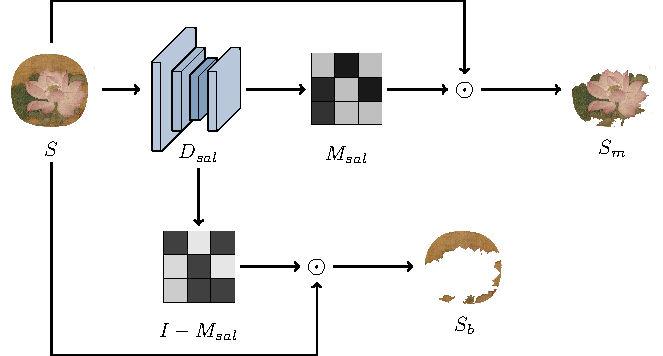
\includegraphics[width=6in]{fig/fig1.pdf}}
    \begin{CJK*}{UTF8}{fs}
        \caption{SS-EPA整体框架。SS-EPA首先将输入图像分成多个补丁,每个补丁线性转换成补丁令牌,并连接一个类别令牌。ViT输出令牌一方面经过重拍列和$1\times 1$卷积生成初始CAM,并由分类层输出分类分数。另一方面经过分割decoder生成语义分割结果。然后从ViT中提取多头自注意力图,并通过HAAF模块进行增强,获取增强补丁语义亲和力。最后通过增强补丁语义亲和力对初始CAM进行优化,并生成伪标签用于监督分割任务。}\label{fig1}
    \end{CJK*}
\end{figure*}

\begin{CJK*}{UTF8}{zhhei}
    \zihao{5}
    \vskip 1mm
    \section{引言}
\end{CJK*}

\begin{CJK*}{UTF8}{fs}
    深度学习推动图像分割显著进步,但依赖精确标注样本,成本高昂。弱监督语义分割(WSSS)技术因此出现,WSSS仅需粗略标注的样本,大幅降低了样本获取的难度。弱监督标注分为边框级标注\cite{39dai2015boxsup,40zhang2021affinity}、涂鸦级标注\cite{41lin2016scribblesup}和图像级标\cite{03ru2023token,12xu2022multi}。其中最难利用的是图像级标注,因为它通常只提供图片的分类标签,包含极少可利用的语义信息,也是多数研究人员最热衷于研究的方法之一。本工作只使用图像级弱标注。

	先前的WSSS方法通常采用多阶段方法,即先训练一个分类网络来生成类激活图Class Activation Map(CAM)\cite{01zhou2016learning},获取类别在图像中的位置信息。然后通过扩展优化CAM生成伪标签,最后利用伪标签全监督地训练语义分割模型。虽然多阶段方法通常可以获得更精准的CAM和更优秀的分割性能,但通常需要分阶段地训练模型和不同的训练策略,耗费大量的计算资源和时间来进行训练和优化,这限制了其在大规模数据集或实时应用中的实用性。通过CNN生成的CAM,存在只激活最显著区域的缺点,原因是CNN感受野有限,对全局信息捕获不完善。Vision Transformer(ViT)\cite{02dosovitskiy2020image}在其它视觉任务中的巨大成功,引起了WSSS领域研究人员的广泛关注\cite{03ru2023token,12xu2022multi,13ru2022learning}。ViT是一种基于 Transformer 架构的视觉模型,它将输入图片划分为小的补丁(patch),并利用Transformer 来建模这些补丁之间的关系。且ViT采用无卷积架构,避免了卷积带来的先验约束,如局部性和平移不变性,使ViT具有更好的可扩展性。基于ViT的WSSS方法首先通过补丁令牌生成粗略的初始CAM,再利用多头自注意力中包含的语义亲和力信息对初始CAM进行优化\cite{12xu2022multi}。然而Transformer中不同深度层的多头自注意力可能关注不同部分,如浅层更关注局部结构、纹理颜色等,深层能捕获更广泛和抽象的视觉语义信息,直接将其与CAM相乘可能会产生错误与误导。且ViT注意力图十分庞大,直接提取所有注意力权重会占据大量计算资源。

	本文提出一种单阶段 WSSS 方法 SS-EPA (Single Stage WSSS with Enhanced Patch Affinity) ,和一种头平均注意力融合增强模块 (Head Average Attention Fusion,HAAF) 。针对先前 CAM 优化多数集中在多阶段方法上的问题,本文提出一种单阶段 WSSS 方法 SS-EPA ,集成了端到端式多头自注意力 CAM 优化方法。 SS-EPA 从 ViT 的自注意力中提取补丁语义亲和力信息,并用于优化初始 CAM 。本文将该端到端的优化方法集成到单阶段 WSSS 方法中,不会影响其完整性和一致性。针对注意力图较为庞大,且不同深度的注意力特性各不相同的问题,本文提出一种头平均注意力融合增强模块 HAAF 。 HAAF 对来自不同层多头自注意力中的语义亲和力进行融合增强,并用于优化从 Transformer 生成的 CAM 。 HAAF 通过对多头自注意力中的各头权重进行平均,聚合不同语义信息,减少不同头重复关注相似区域的冗余信息。随后,通过全局平均池化聚合每个注意力图的全局特征,并将其输入多层感知机,提取更复杂的特征关系。最终获得融合后的增强注意力图,充分考虑了不同层次注意力的重要性。 HAAF 可以去除头重复关注、包含无效信息的冗余问题,显著降低计算资源消耗并提升效率。该方法还能减少每个头对噪声或异常的敏感度,提高模型鲁棒性。

	为了验证本文提出的 SS-EPA 和 HAAF 模块的有效性,本文在 Pascal VOC 2012数据集上评估了SS-EPA的CAM、伪标签和分割结果的性能表现,并与基线方法ToCo\cite{03ru2023token}相比较。对比实验、消融实验以及各种可视化结果表明,本文所提方法可以显著优化生成的CAM,伪标签和分割模型误分类的概率更小,且有更加完整和准确的对象边界。在VOC验证集上与基线相比,伪标签和分割性能分别提升了2.2\%和1.3\%的mIoU分数,充分验证了本文方法的有效性。

    总的来说,本文主要贡献包括以下三个方面:
    \begin{itemize}
        \item 提出了一种名为 SS-EPA 的单阶段 WSSS 方法,集成了端到端式多头自注意力 CAM 优化方法。在不影响单阶段方法的完整性和一致性的前提下,集成了利用补丁语义亲和力信息优化初始 CAM 的方法,使 CAM 更加精细和准确,从而生成更加优质的伪标签用于训练分割模型。
        \item 提出一种头平均注意力融合增强模块(HAAF),来解决语义亲和力信息包含噪声与错误,以及注意力图较为庞大的问题。通过对注意力的不同头的权重做平均,HAAF可去除冗余信息并提高模型鲁棒性,利用多层感知机的交互能力,HAAF可以充分考虑来自不同层注意力的重要性,对包含语义亲和力的自注意力完成简化和增强。
        \item 在 Pascal VOC 2012 数据集上的实验表明,本文方法可以显著优化生成的 CAM ,最终的分割模型性能相比以前的单阶段方法有了实质性的改进,且实现了与一些多阶段方法相当的性能。
    \end{itemize}
\end{CJK*}

\section{Traditional Style Transfer}

The term "style transfer" is usually used to refer to the second phase of neural style transfer that began after the publication of Gatys et al.'s paper in 2016 \citep{02gatys2016image}. Before this, the term "style transfer" was not widely accepted. The work in the first phase is often referred to as Non-Photorealistic Rendering (NPR) or Image-Based Artistic Rendering (IB-AR).

In this paper, we refer to the work from the first phase (1990s-2016) as traditional style transfer to help readers better understand the continuity between the two approaches. We follow the suggestion from \citep{01jing2019neural} and adopt the classification method for traditional style transfer proposed in \citep{21kyprianidis2012state}. However, the focus of this paper is not on traditional style transfer, especially since traditional methods have now been largely integrated with neural style transfer techniques. Therefore, we recommend readers who require a systematic understanding of traditional style transfer methods to refer to these two works\citep{01jing2019neural,21kyprianidis2012state}.

When introducing the achievements of traditional style transfer, this paper will proceed by discussing their characteristics, advantages, and limitations.

\textbf{Stroke-Based Rendering (SBR)}is a core algorithm in traditional style transfer that involves covering a 2D canvas with atomic-level rendering primitives to simulate specific artistic styles. These primitives typically include virtual brushstrokes, patches, stippling, and shading marks.

The most common form of SBR is rendering with virtual brushstrokes. The color, direction, size, and order of these strokes may be determined semi-automatically or automatically. The stylized output depends not only on the simulation of the medium used to render each stroke but also on the process of stroke placement and the methods used to set their attributes. The stroke placement process in SBR can be roughly divided into local and global approaches. Local methods typically base stroke placement decisions on the pixels within the spatial neighborhood of the stroke. This can be explicitly specified in the algorithm (e.g., image moments within a window) or implied by previous convolution operations (e.g., Sobel edges). A branch of SBR uses media other than colored pixels or paint to fill image regions, including using small dots (stippling) for tone description, line patterns or curves (shading marks), and mosaic algorithms that combine small tiles. When handling video content, the motion of the strokes should match the movement in the video content. This is particularly emphasized in SBR algorithms to ensure dynamic effects and visual coherence in videos. The advantage of SBR lies in its ability to create effects that closely resemble traditional artworks, making it especially suitable for mimicking styles such as oil painting, watercolor, and sketching. However, SBR methods may struggle when dealing with highly complex or abstract artistic styles, as these styles may not be easily achieved through traditional stroke simulation.


\textbf{Example-Based Rendering (EBR)}is a technique aimed at learning and mimicking specific artistic styles. It does so by analyzing the mapping relationship between an example pair (e.g., an original image and an artist's rendered version of that image) and then applying this mapping to stylize other images. Such methods typically encode a set of heuristic rules to faithfully depict the intended style. They try to capture the essential characteristics of a style by learning and imitating the techniques and styles an artist applied in a particular work. Once the mapping is learned, it can be used to stylize arbitrary images, making them visually similar to the original example images. This approach not only mimics specific artistic styles but can also replicate the unique style of a particular artist. The advantage of EBR is that it can produce highly personalized results, making it particularly suitable for imitating the style of specific artists or works. However, this method depends heavily on high-quality example pairs, and it may be difficult to achieve the desired stylization effect if suitable training data is lacking.

\textbf{Image Processing and Filtering (IPF)}is based style transfer uses various image processing filters and algorithms to achieve artistic stylization. This includes techniques that are based on image pyramids, as well as the use of interactive techniques (such as human gaze trackers and saliency maps) to explore different levels of an image. Various filtering techniques explore different image processing filters used for artistic stylization, but to date, only a few results have been considered interesting from an artistic perspective. This may be because these filters usually focus on the restoration and enhancement of photorealistic images. The image pyramid and interactive techniques (such as human gaze trackers and saliency maps) explore hierarchical representations by segmenting different resolution versions of the source image. High-level abstraction is achieved by rendering only the coarse large regions or specific areas located at the top of the pyramid. This method helps capture larger shapes and compositional features in the image, rather than detailed textures or lines. Unlike the simplification typically pursued in Image-Based Artistic Rendering (IB-AR), these filtering methods are often associated with the restoration and enhancement of photorealistic images. The advantage of this approach lies in its ability to quickly and easily apply stylization to images, making it suitable for creating diverse and abstract visual effects. However, such methods lack the fine detail and complexity required for artistic stylization, making it difficult to precisely mimic the subtle features of specific artists or styles.

\textbf{Summary}\quad As pioneers in the field of style transfer, these methods have inspired the emergence and development of neural style transfer, but they share some common shortcomings. Each different style transfer method embodies the author's understanding of a particular style. However, because these methods often incorporate the author's interpretation of the style, the transfer results may be correlated with the author's aesthetic level, leading to varying quality in the stylized output. Additionally, the algorithms designed for the same or similar textures or styles are often similar or even identical, resulting in stylized images with textures that may appear rigid and dull. The limited generalization capability also restricts the broad application of traditional style transfer methods. Traditional methods are designed for specific types of styles and images, and their effectiveness diminishes when generalized to different styles or images.

\section{Neural Style Transfer}

The technique of using neural networks for style transfer is generally referred to as neural style transfer. It is widely acknowledged that the concept of neural style transfer began to gain traction after Gatys et al.\citep{02gatys2016image} utilized convolutional neural networks (CNNs) for style transfer. This paper draws on some of the classification perspectives of neural style transfer discussed in \citep{01jing2019neural}, and based on the current developments in the field and personal understanding, modifies and adds to these perspectives to form a new classification standard for neural style transfer. The new classification standard is primarily based on three criteria: the developmental stages of neural style transfer, the main issues explored at different stages, and the different approaches to solving these issues.

Under this standard, this paper divides neural style transfer into three developmental stages:
\begin{enumerate}
    \item Early Stage: Online style transfer based on pixel iteration, led by Gatys et al. \citep{02gatys2016image}.
    \item Developing Stage: Offline style transfer based on model iteration, led by Johnson et al.\citep{22johnson2016perceptual} and Ulyanov et al.\citep{23ulyanov2016texture}.
    \item Current Stage: Arbitrary and efficient style transfer.
\end{enumerate}

Dividing neural style transfer into these three stages reflects more effectively the developmental trajectory of the field of neural style transfer, allowing researchers to clearly understand the reasons for the emergence of each stage, the main issues being explored, and the solutions proposed. It is important to note that the chronological classification used in this paper may not always accurately place certain works within a specific stage, as some contributions lie at the intersection of two stages and exhibit characteristics of both. In such cases, this paper classifies them into the earlier stage to highlight their connection to preceding work.

Each of the three stages mentioned above has corresponding subcategories. For online style transfer based on pixel iteration, it can be further categorized into two types based on the type of loss function used: style transfer based on parametric models and style transfer based on non-parametric models. For offline style transfer based on model iteration, it can be classified according to the network and the number of styles that can be transferred by the network, resulting in two subclasses: single-network model generating single style, and single-network model generating multiple styles. For arbitrary and efficient style transfer, based on the different technologies used to achieve style transfer, it can be divided into two categories: those that build their own network frameworks and those that use other emerging technologies as support.

This paper will introduce the contributions of each stage of neural style transfer according to the above classification standard. For each contribution, the paper will first provide a brief introduction to its underlying concept, followed by an analysis of its advantages and disadvantages, leading into the next contribution. The categories of neural image style transfer is illustrated as Figure \ref{fig1}

\subsection{Pixel-Iterative Online Style Transfer}

Pixel-iterative online style transfer can be traced back to the research of Alexander et al. \citep{24mordvintsev2015inceptionism} on Convolutional Neural Networks (CNNs). Alexander et al. \citep{24mordvintsev2015inceptionism} aimed to investigate why CNNs have the ability to extract image features. To this end, they inverted a CNN and used the inverted CNN to reverse-engineer the feature maps extracted by the original CNN, attempting to reconstruct an image similar to the original one. As described by Alexander et al. in their paper \citep{24mordvintsev2015inceptionism}, they were able to generate images with "certain artistic characteristics" through this method, as illustrated in Figure \ref{fig2}.


\begin{figure}[htbp]%% placement specifier
    %% Use \includegraphics command to insert graphic files. Place graphics files in 
    %% working directory.
    \centering%% For centre alignment of image.
    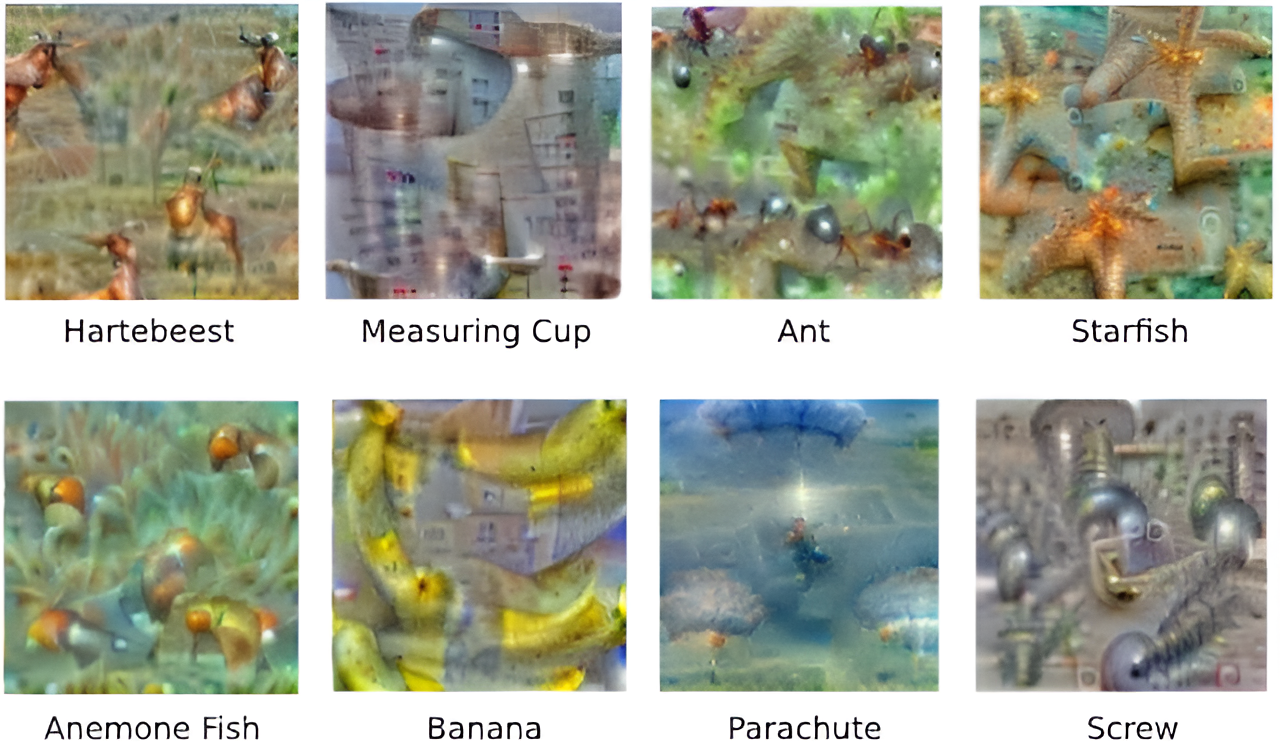
\includegraphics[width=0.95\textwidth]{fig/Alex_classvis.png}
    %% Use \caption command for figure caption and label.
    \caption{The Artistic Images Generated by Alexander et al.\citep{24mordvintsev2015inceptionism}}\label{fig2}
    %% https://en.wikibooks.org/wiki/LaTeX/Importing_Graphics#Importing_external_graphics
\end{figure}


Through the aforementioned experiment, DeepDream discovered that CNNs could not only extract image features but also generate images. This concept of "using neural networks for feature extraction followed by other methods for image generation" laid a foundational groundwork for the subsequent use of neural networks in style transfer.

Following DeepDream, Gatys et al. \citep{02gatys2016image} in 2016 combined deep learning with style transfer in a groundbreaking manner, significantly advancing the effectiveness of style transfer and reaching new heights in visual quality.

This paper posits that if a style transfer method uses a content image and a style image as inputs, and iteratively processes a noise image at the pixel level during the generation of a stylized image, resulting in the final output of a stylized image, then this approach can be classified as pixel-iterative style transfer. Furthermore, depending on the implementation method, this category can be further subdivided into parametric model-based style transfer and non-parametric model-based style transfer.

\subsubsection{Parameterized Model-Based Style Transfer}

The work of Gatys et al. \citep{02gatys2016image} can be regarded as the first use of a parametric model for style transfer, and it is also considered the first significant achievement in the entire field of neural style transfer.

In their 2016 paper\citep{02gatys2016image}, Gatys et al. were the first to combine Convolutional Neural Networks (CNNs) with style transfer. The idea behind this achievement originated from the discovery of Gatys et al. during their research on CNNs: a CNN trained with sufficient data can extract features across different datasets\citep{02gatys2016image}. In the realm of style transfer, this capability of CNNs to extract features can be used to capture the content features of a photograph as well as the style features of an artwork. Figure \ref{fig3_VGGs_Ability} illustrates how the VGG16 image classification network, based on CNNs, is capable of extracting both content and style features at different layers of the network.

\begin{figure}[!htbp]%% placement specifier
    %% Use \includegraphics command to insert graphic files. Place graphics files in 
    %% working directory.
    \centering%% For centre alignment of image.
    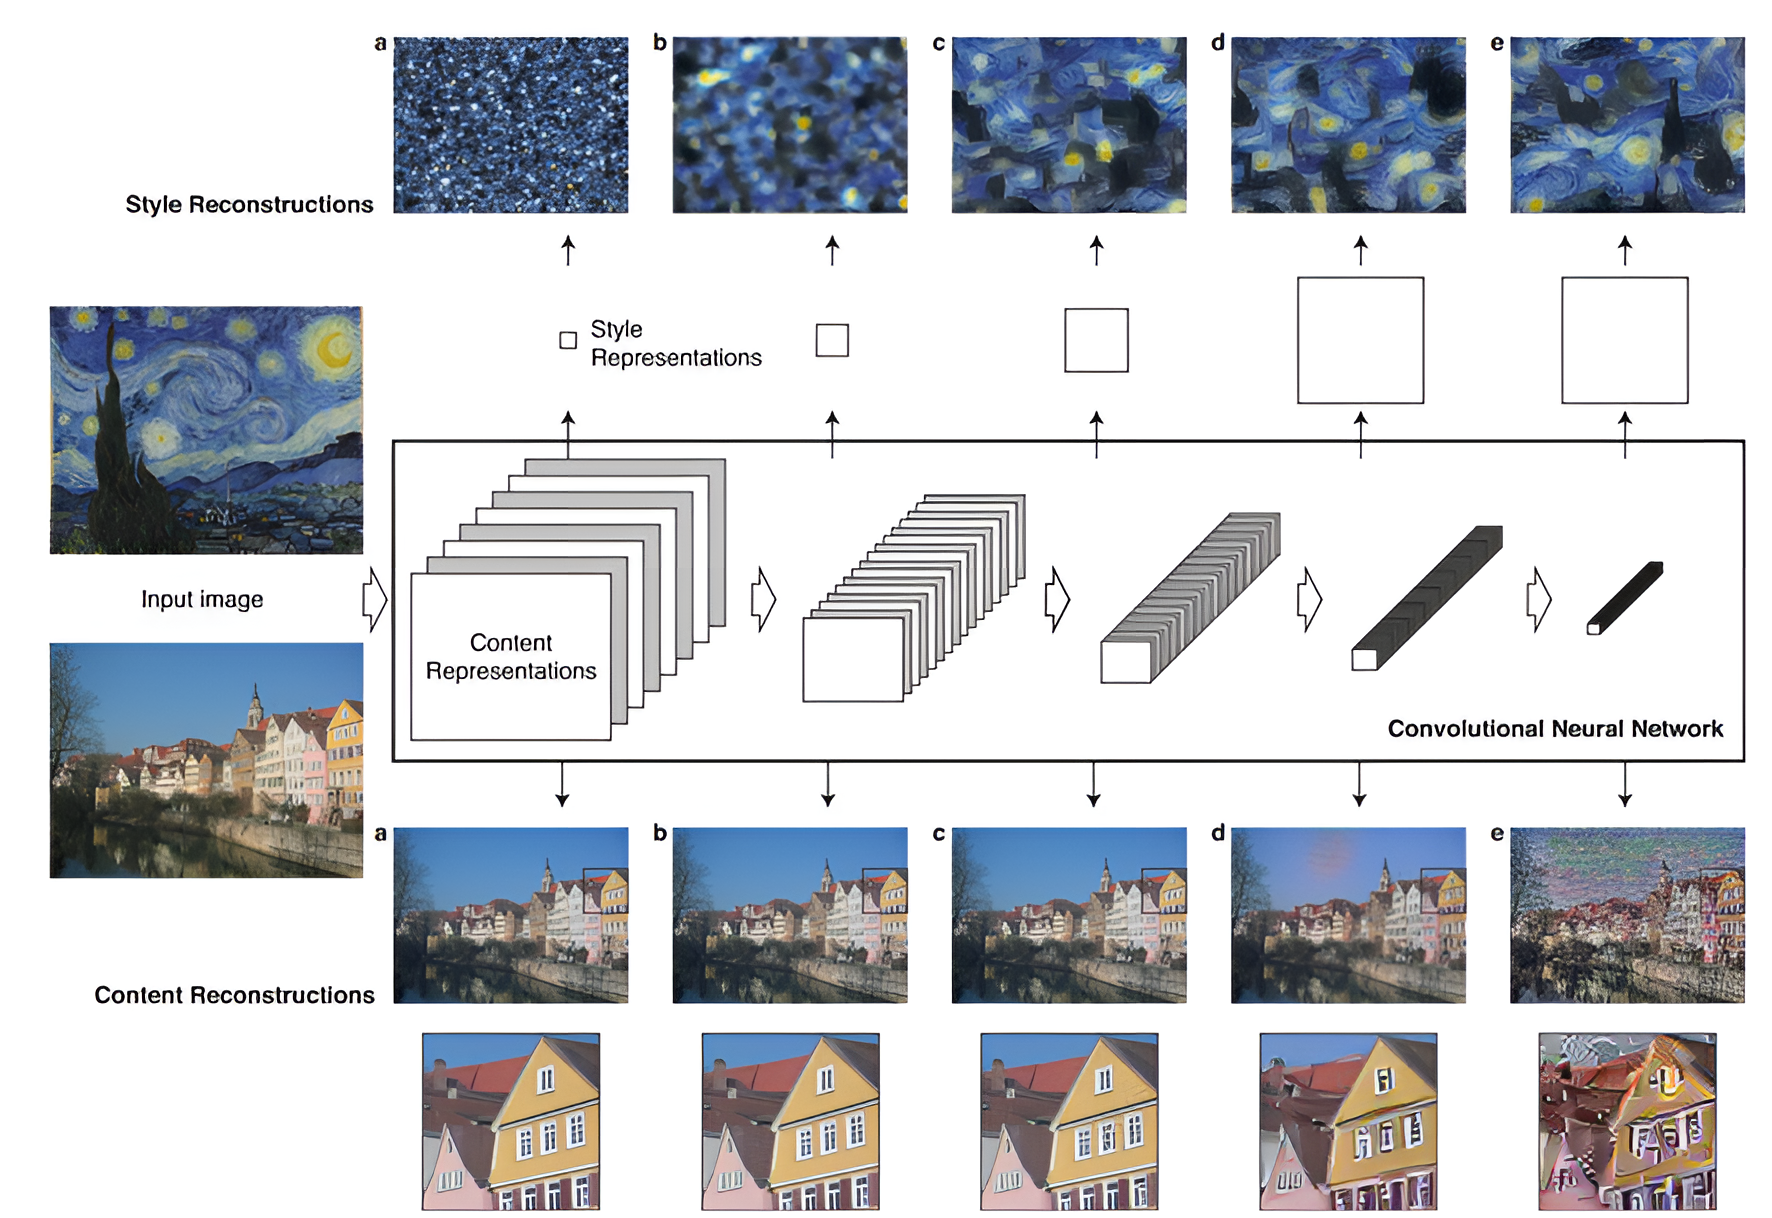
\includegraphics[width=0.95\textwidth]{fig/VGGs_Ability.png}
    %% Use \caption command for figure caption and label.
    \caption{CNN Can Extracting Both Content and Style Features}\label{fig3_VGGs_Ability}
    %% https://en.wikibooks.org/wiki/LaTeX/Importing_Graphics#Importing_external_graphics
\end{figure}

In terms of practical implementation, Gatys et al.\citep{02gatys2016image} achieved style transfer by defining a loss function and using it to optimize a noise image. This loss function is based on the differences between high-level features of the content image and the image being stylized, as well as the differences between high-level features of the style image and the image being stylized. Guided by this loss function, the noise image is iteratively optimized until the loss function reaches its minimum, resulting in the final stylized image. The specific form of the loss function is as follows:

\begin{equation}
    \label{Gatys_total_loss}
    L_{total}=\alpha L_{content}+ \beta L_{style}
\end{equation}

where $L_{total}$  is the overall loss function, $L_{content}$ is the content loss, which measures the degree of content difference between the stylized image and the content image, and $L_{style}$  is the style loss, which measures the degree of style difference between the stylized image and the style image. $\alpha$ and $\beta$ are hyperparameters used to control the similarity between the generated stylized image and the content image and the style image, respectively. Specifically, the content loss function $L_{content}$  is expressed as follows:

\begin{equation}
    \label{gatys_content_l}
    L_{content}\left(\vec{p},\vec{x},l\right)=\frac{1}{2} \sum_{i,j} \left(F_{ij}^l-P_{ij}^l\right)^2
\end{equation}

where $\vec{p}$ is the flattened input of the content image, input into the network in vector form;$\vec{x}$ is the stylized image, which also needs to be flattened for processing. $l$ represents the $l$-th layer in the network.$F^l$ denotes the set of all feature maps generated by the $l$-th layer of the network for the image undergoing style transfer, and $F_{ij}^l$ refers to the value at position $j$ in the flattened vector of the $i$-th feature map in the set $F^l$ generated by the VGG \citep{25simonyan2014very} network at layer $l$. Similarly, $P^l$ denotes the set of all content feature maps generated by the $l$-th layer of the network for the input content image, and $P_{ij}^l$ refers to the value at position $j$ in the flattened vector of the $i$-th content feature map in the set $P^l$. The formula's purpose is to calculate the pixel-wise difference between the feature maps of the stylized image and the corresponding feature maps of the content image, summing these differences. Gradient descent and other optimization methods are used to minimize this value until it stabilizes at a small value.

On the other hand, before providing the specific expression of the style transfer function $L_{style}$ , it is necessary to introduce its core component—the Gram matrix. To extract the style features of the input image, Gatys et al.\citep{02gatys2016image} used a feature space designed to capture texture information, which is built on the output of any convolutional layer in the network. This feature space is constructed from the correlations between feature maps of different convolutional layers, with these correlations represented by the inner product of the $i$-th and $j$-th vectorized feature maps in the $l$-th layer. This inner product is known as the Gram matrix, denoted as $G^i \in R^{N_l\times N_l}$. The formula for the Gram matrix is as follows:
\begin{equation}
    G_{ij}^l=\sum_k F_{ik}^lF_{jk}^L
\end{equation}

Based on the Gram matrix, Gatys et al.\citep{02gatys2016image} processed the noise image using gradient descent and aimed to minimize the mean squared distance between the Gram matrix of the original image and the Gram matrix of the style image. The contribution of the $l$-th layer in the network to the style loss function $L_{style}$  is as follows:
\begin{equation}
    \label{Gatys_style_loss_l}
    E_l = \frac{1}{4N_l^2M_l^2}\sum_{ij}\left(G_{ij}^l-A_{ij}^l\right)^2
\end{equation}
where $N_l$ represents the number of convolutional kernels in a convolutional layer of the network, which is also the number of feature maps that the layer can generate. $M_l$ is the number of pixels contained in each feature map, numerically equal to the product of the height and width of the feature map.$A_{ij}^l$ and $G_{ij}^l$ represent the pixel values at position $j$ in the $i$-th vectorized feature map at layer $l$ of the network. Formula \ref{gatys_style_l} only computes the contribution of a single layer to the style loss $L_{style}$ . The overall style loss $L_{style}$  is obtained by summing the weighted losses from all layers, with the specific formula as follows:

\begin{equation}
    \label{gatys_style_l}
    L_{style}\left(\vec{a},\vec{x}\right)=\sum_{l=0}^L \omega_l E_l
\end{equation}
where $w_l$ is the weight representing the impact of each layer on the total style loss function, and $L$ is the number of convolutional layers in the network. By taking the partial derivative of Formula \ref{Gatys_total_loss}, $\frac{\partial L_{total}}{\partial \vec{x}}$ is obtained, which can be used as input for optimization algorithms and guide the iterative processing of the stylized image to achieve style transfer.

The parameterized model style transfer method based on the Gram matrix introduced by Gatys et al. has distinct advantages\citep{02gatys2016image}. Compared to traditional style transfer methods, it overcomes the limitations of rigid and less variable brushstrokes and achieves excellent results. It also addresses the limitation of traditional methods being restricted to specific styles, enabling the transfer of natural and stylized textures\citep{01jing2019neural}, thus achieving good transfer results. However, this method has some notable drawbacks. Since style transfer starts from a noise image each time, it requires a significant amount of time for batch processing and performs poorly in real-time style transfer. Additionally, the Gram matrix is more adept at capturing global information of feature maps, leading to unsatisfactory results in extracting regular textures with long-range symmetrical structures\citep{01jing2019neural}. Moreover, unlike traditional methods that ignore high-level semantic information, Gatys et al.\citep{02gatys2016image} considered only high-level semantic information and neglected low-level semantic information, resulting in deficiencies in the fine structure and detail coherence of the synthesized stylized images.

To address the shortcomings of fine texture handling in Gatys et al.'s method, Berger et al.\citep{26berger2016incorporating} proposed horizontal and vertical pixel differences, focusing on examining the differences between each pixel and other pixels in its horizontal and vertical directions. In practice, this method calculates the feature relationships between the pixel located at position $(i, j)$ and pixels at positions $(i,j+\delta)$ or $(i+\delta,j)$ in the feature map, incorporating these into the style loss consideration. This approach allowed Berger et al.\citep{26berger2016incorporating} to achieve effective transfer of symmetric long texture patterns, somewhat compensating for Gatys et al.'s limitations in simulating fine structures and regular textures with long-range symmetry. However, since the method still relies on the Gram matrix as the core of style transfer, it retains some of the shortcomings of Gatys et al., such as inadequate texture detail simulation and unstable style transfer quality.

To investigate the reasons behind the style instability in images generated using the Gram matrix, Risser et al.\citep{27risser2017stable} conducted a further in-depth study of Gatys et al.\citep{02gatys2016image}. Risser et al. proposed that the instability in generated image styles is due to feature maps with different means and variances potentially having the same Gram matrix. Based on this finding, Risser et al. incorporated histograms of feature maps into the style transfer loss function, further optimizing the Gram matrix-based style transfer method. The advantage of this approach is the generation of more stable style images; however, incorporating histograms of feature maps makes the computation more complex, increasing the time required for style transfer and reducing efficiency in batch processing. Moreover, Risser et al. only addressed the stability of generated images, leaving the issue of detailed texture description unresolved.

Li et al.\citep{28li2017demystifying} attempted to explain the principles of neural style transfer using more mature domain knowledge, considering neural style transfer as a special variant of domain adaptation tasks. From this perspective, Li et al. provided a different viewpoint. Domain adaptation tasks are based on the fact that the distributions of source and target data are different, with the goal of training a model on a labeled source domain dataset to predict the target domain data distribution. One method of domain adaptation is to minimize the distribution difference between source and target domain samples, where Maximum Mean Discrepancy (MMD) is a commonly used measure. Analogously, in style transfer tasks, the content image can be considered as the source domain, and the stylize image as the target domain. Li et al. explored the mathematical role of the Gram matrix in style transfer and proved that the process of matching Gram matrices of style images and stylized images (i.e., Formula \ref{Gatys_style_loss_l}) is essentially equivalent to minimizing an MMD with a quadratic polynomial kernel. Therefore, Li et al. proposed that minimizing MMD with other kernels (such as linear, polynomial, or Gaussian kernels) might be useful in style transfer. The main contribution of Li et al. is that they provided a theoretical exploration and clarification of the principles of Gatys et al.\citep{02gatys2016image}.

The aforementioned parameterized model-based neural style transfer methods have some common defects. Due to the loss of low-level information in convolutional neural networks, the transfer results for objects with regular shapes (e.g., man-made objects) often exhibit noticeable distortions. Although Berger et al.\citep{26berger2016incorporating} made contributions in this area, there is still significant room for improvement. Additionally, the style transfer process is time-consuming, requiring substantial time for batch processing of many images, and thus is less efficient in tasks with large numbers of images, such as video style transfer. The generated style is also unstable and lacks temporal consistency.

\subsubsection{Non-Parametric Model-Based Style Transfer}

Markov Random Fields (MRFs) are a primary method used in non-parametric model-based neural style transfer\citep{29li1994markov,30cross1983markov,31chellappa1985texture,32bennett1998multispectral}. The use of MRFs for texture synthesis is also a common technique in traditional style transfer methods. Li and Wand \citep{33li2016combining} chose to integrate the traditional MRF-based method into neural style transfer. In their work \citep{33li2016combining}, they combined MRFs with deep convolutional neural networks (dCNNs) and proposed a non-parametric neural style transfer method. They argued that the parameterized style transfer method using Gram matrices only considers differences between pixels and lacks spatial-level constraints on the stylized image, leading to insufficient realism in the generated images. Therefore, Li and Wand replaced the Gram matrix with an MRF regularizer and introduced a new loss function:

\begin{equation}
    L_s=\sum_{l\in {l_s}}\sum_{i=1}^m \mid\mid\Psi_i(F^l(I))-\Psi_{NN(i)}(F^l(I_s))\mid\mid^2
\end{equation}
where $\Psi(F^l(I))$ represents the set of all local patches in the feature map$F^(I)$; $\Psi_i(F^l(I))$ refers to the $i$-th local patch within this set; $\Psi_{NN(i)}$ is the style patch in the stylized image $I$ that most closely matches the $i$-th local patch in terms of style similarity. This best-matching stylized patch $\Psi_{NN(i)}$ can be found by calculating the normalized correlation between all style patches in the style image. Here, $m$ denotes the total number of local patches. The method proposed by Li and Wand improved upon the style transfer results achieved by Gatys et al.\citep{02gatys2016image}, making the structures in the stylized images more coherent and better preserving the fine details of the original image, leading to significant progress in synthesizing realistic photos. However, this method lacks attention to the semantic content of the images. If there is a substantial structural difference between the content and style images, the matching between local patches and style patches might not be accurate, resulting in poor quality of the generated stylized images.

\textbf{Summary}\quad The pixel-iteration-based style transfer methods can be considered as early explorations in the field of neural style transfer, holding a pioneering position.
Neural style transfer technology overcomes the limitation of traditional style transfer techniques, which only transfers a single style. It has better generalization ability, achieving a "once-for-all" approach to some extent, meaning that once a network structure is built, it can transfer any style and handle images of any resolution. Additionally, thanks to the CNN's feature extraction capabilities, neural style transfer can capture advanced artistic styles and textures, exhibiting flexible and diverse texture features within the same stylized image.
However, despite the groundbreaking achievements of pixel-iteration-based style transfer, some common issues cannot be ignored, with the most critical being resource consumption and time expenditure. Pixel-iteration-based style transfer requires multiple iterations of a noise image under the guidance of a loss function, with each iteration involving feature extraction and computation by a CNN. As a result, a significant amount of computational resources and time is consumed during the image generation stage. For instance, when transferring the style of a $512\times 512$ image to generate a similarly sized stylized image, the process can take up to 51.19 seconds\citep{01jing2019neural}. If one attempts to transfer a high-resolution (e.g., 4K) image, the time required becomes even more prohibitive for practical applications.
Moreover, even after investing substantial time and computational resources in style transfer, it is often difficult to consistently achieve results that surpass those of traditional style transfer methods.
These two major drawbacks have hindered the widespread application of neural style transfer technology in real-world scenarios, leading to a stagnation in the research of neural style transfer. 



\subsection{Model-Iteration-Based Offline Style Transfer}

As previously mentioned, although pixel-iteration-based style transfer methods have the ability to perform arbitrary style transfers, their low efficiency prevent them from being widely used in real-life scenarios, especially when dealing with tasks involving a large number of images. This drawback is particularly evident in such cases. To improve the efficiency of neural style transfer, researchers have developed fast-style transfer methods that trade off either the quality of style transfer or the number of transferable styles. These methods are referred to as model-iteration-based style transfer.

Generally, the primary approach to achieving model-iteration-based style transfer is to shift the time required during inference to the training phase. Specifically, this is typically done by training a specific style transfer network, which stores style information in the form of parameters within the network. When confronted with different styles, the network can quickly retrieve the corresponding parameters, thereby enabling fast style transfer.

From a historical perspective, model-iteration-based style transfer can be divided into two stages: the first stage involves a single model generating a single style, and the second involves a single model generating multiple styles. To help readers accurately classify the methods used in the literature, this paper provides detailed descriptions of these two categories: if a style transfer method takes a content image as input and the network can quickly convert it into a specific stylized image, the method can be classified as Per Model Per Style transfer. On the other hand, if a style transfer method takes a content image and the encoded representation of the desired final style as input, and the network can quickly convert it into a stylized image corresponding to the style code, the method can be classified as Per Model Multi Style transfer. 

\subsubsection{Per Model Per Style}

\textbf{Using feedforward networks to achieve Per Model Per Style.} Johnson et al.\citep{22johnson2016perceptual} and Ulyanov et al.\citep{23ulyanov2016texture} were the first to publish work on real-time style transfer. Independently, in 2016, they both proposed methods for real-time style transfer using feedforward neural networks. The main idea was to train a feedforward neural network that encodes style information in the network's parameters, allowing the generation of stylized images without the need for multiple iterations of optimization on a noise image. Specifically, the following feedforward neural network needs to be trained: 
\begin{equation}
    \begin{aligned}
        \theta^* &= \arg\min L_{total}\left(I_c,I_s,g_\theta*(I_c)\right),\\
        I^*&=g_\theta*(I_c),
    \end{aligned}
\end{equation}
where $\theta^*$ represents the optimal parameters that minimize the total loss function $L_{total}$.

The total loss function $L_{total}\left(I_c,I_s,g_\theta*(I_c)\right)$ evaluates the quality of the style transfer. This function has three inputs: the content image $I_c$, the style image $I_s$, and the stylized image $g_\theta*(I_c)$. It produces a single output, $I^*$, which is the final stylized image. The goal of this function is to find the parameters $\theta^*$ that minimize $L_{total}$. These parameters are used to transform the content image $l_c$ into the final stylized image $I^*$.
\begin{figure}[!htbp]%% placement specifier
    %% Use \includegraphics command to insert graphic files. Place graphics files in 
    %% working directory.
    \centering%% For centre alignment of image.
    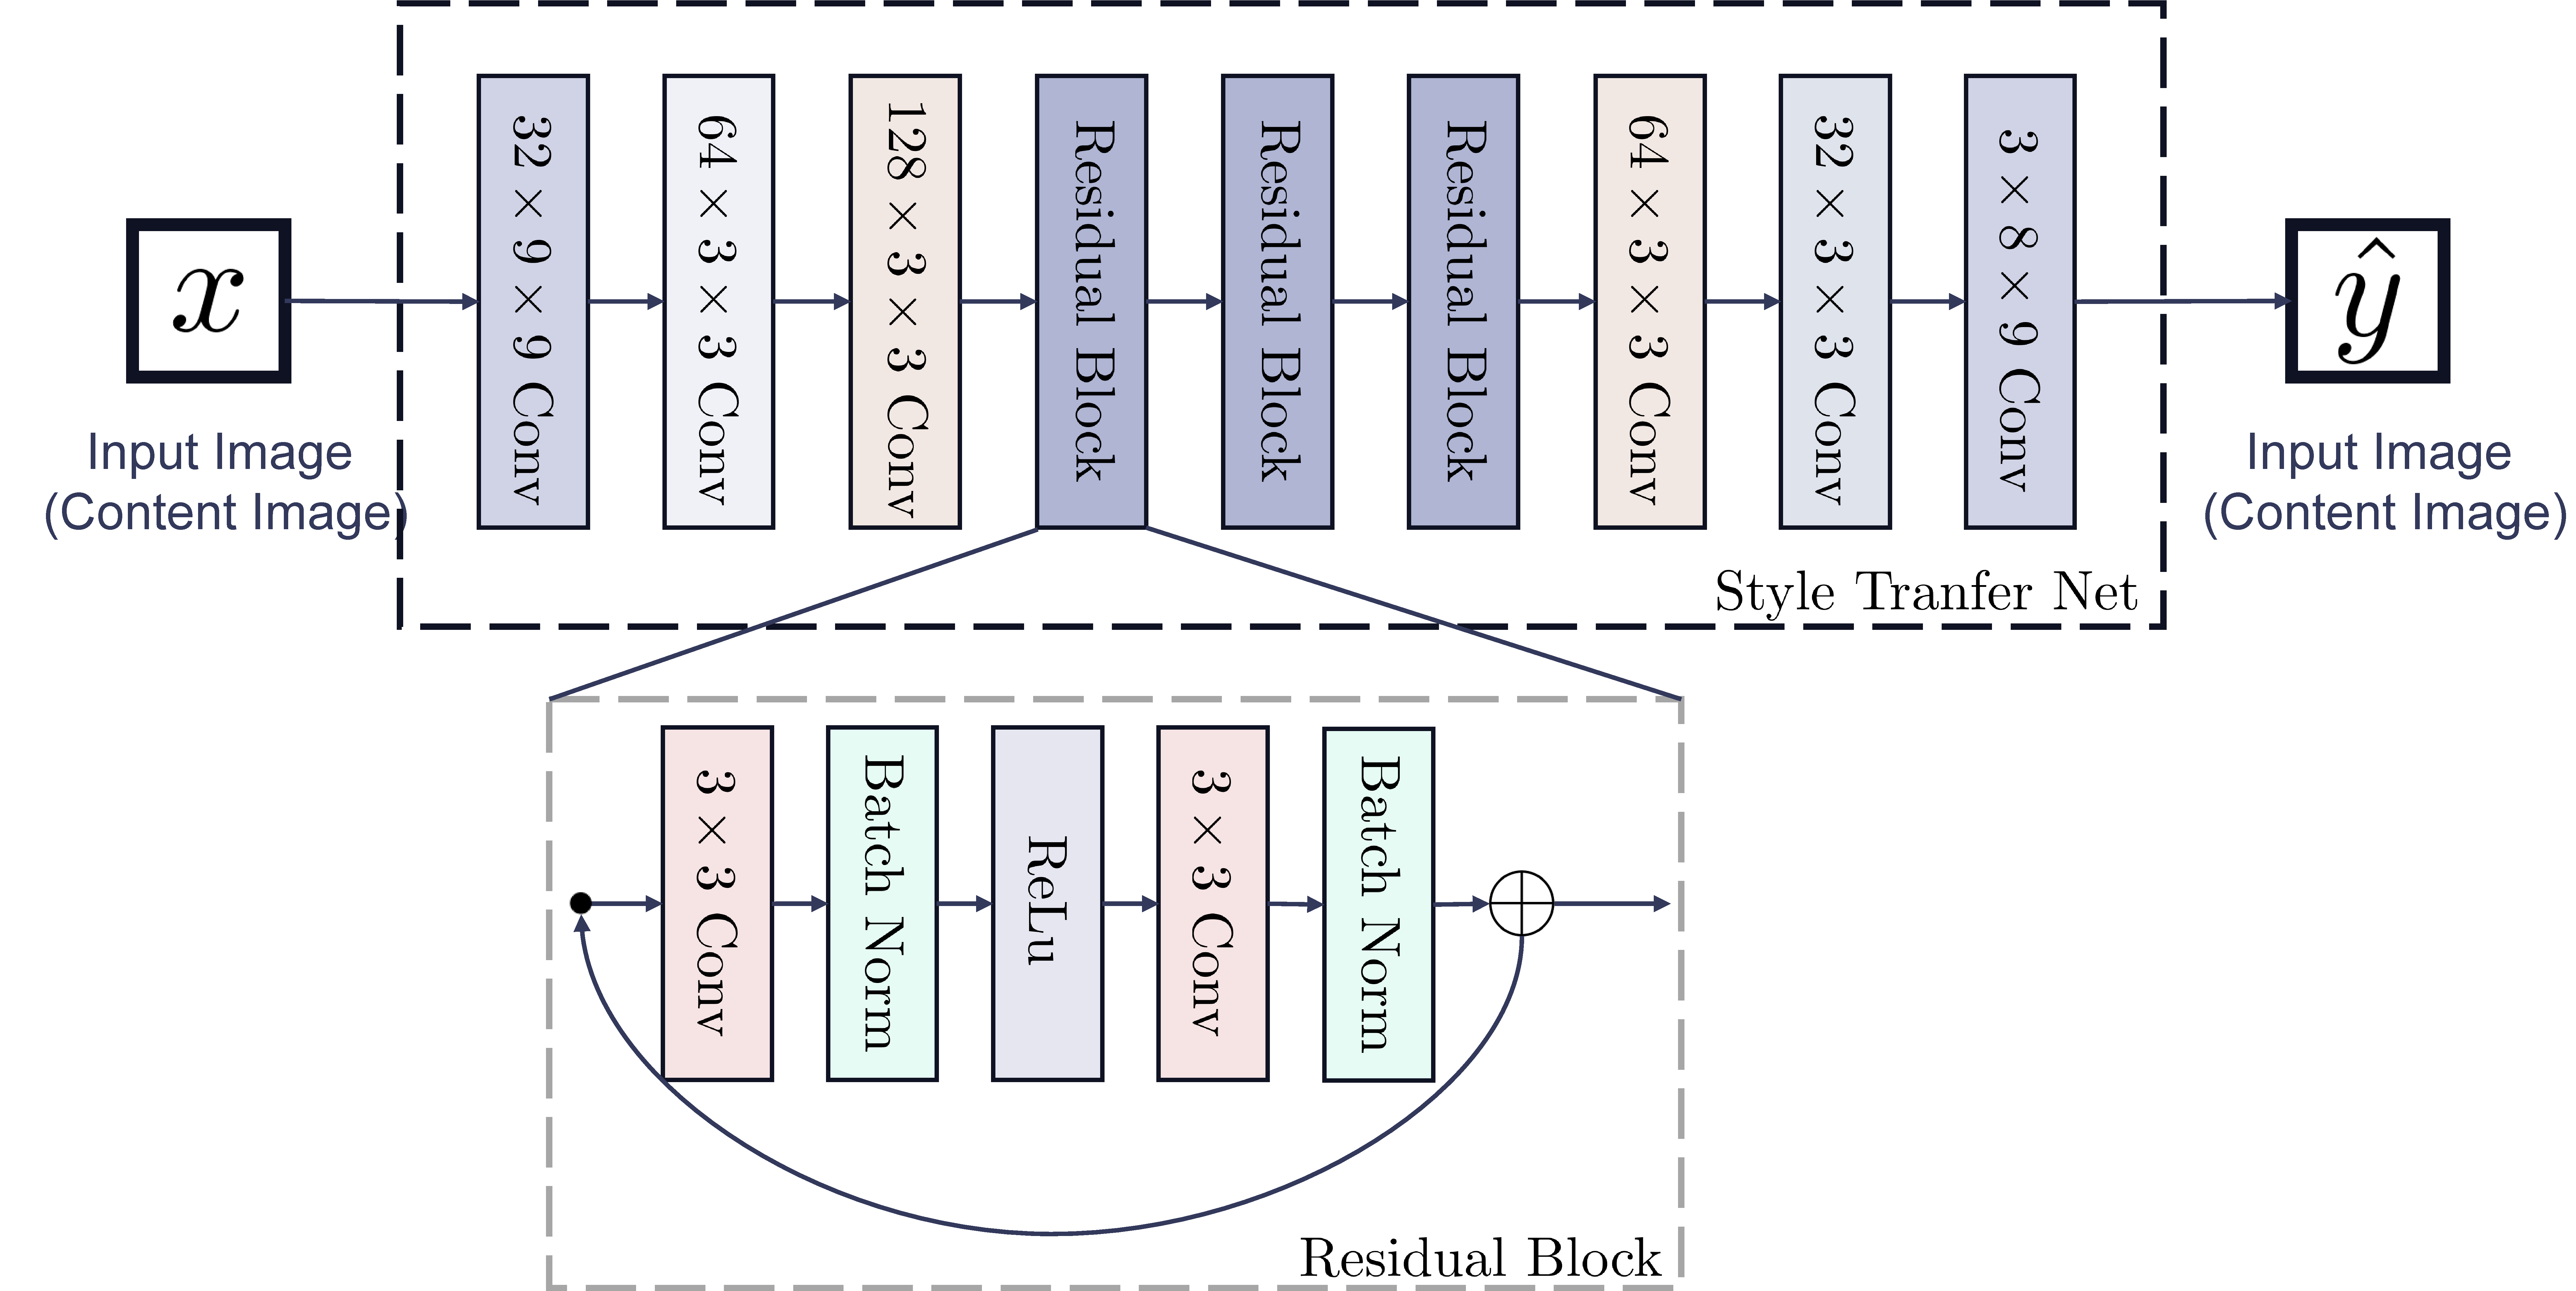
\includegraphics[width=0.95\textwidth]{fig/Figure_3_Johnson_et_al's_Network_Architecture_[22].pdf}
    %% Use \caption command for figure caption and label.
    \caption{Johnson et al.'s Network Architecture \citep{22johnson2016perceptual}}\label{fig4_Johnson}
\end{figure}

Although Johnson et al. and Ulyanov et al. proposed this method simultaneously, there are differences in their network structures. Johnson\citep{22johnson2016perceptual} et al. built upon the method by Radford et al.\citep{34radford2015unsupervised}, adding residual blocks and step-wise convolution, and introduced an Instance Normalization (IN) layer to accelerate the network's convergence, as shown in Figure \ref{fig4_Johnson}.


On the other hand, Ulyanov et al.\citep{23ulyanov2016texture} used a multi-scale structure as the generative network (as shown in Figure \ref{fig5_Ulyanov}), with an objectiveKwo function similar to that of Gatys et al.\citep{02gatys2016image} Both Johnson et al. and Ulyanov et al. based their methods on feedforward generative networks, achieving real-time style transfer. Compared to the method by Gatys et al.\citep{02gatys2016image}, the speed of style transfer was improved by two orders of magnitude.

\begin{figure}[!htbp]%% placement specifier
    %% Use \includegraphics command to insert graphic files. Place graphics files in 
    %% working directory.
    \centering%% For centre alignment of image.
    \includegraphics[width=0.95\textwidth]{fig/Figure_4_Ulyanov_et_al_'s_Network_Architecture_[23].pdf}
    %% Use \caption command for figure caption and label.
    \caption{Ulyanov et al.'s Network Architecture\citep{23ulyanov2016texture}}\label{fig5_Ulyanov}
\end{figure}

However, since both methods during training largely follow the approach proposed by Gatys et al., they encounter similar issues in migration effects, such as unsatisfactory results in image detail and structural consistency.

\textbf{Using Markov Random Fields for Per Model Per Style.}\quad The use of Markov Random Fields can also enhance the speed of style transfer. Li and Wand et al.\citep{35li2016precomputed} improved their previous work\citep{33li2016combining} by obtaining a Markov feedforward network through adversarial training (Figure 5), thereby addressing the efficiency problem. In principle, this method is similar to their earlier non-parametric style transfer approach based on image patches described in\citep{33li2016combining}. This improvement allows them to achieve better results in object structure consistency, thereby preserving the fine details of the original image more effectively. However, some shortcomings of the original methods remain, such as poor performance when the matching between local patches and style patches is not precise.

\begin{figure}[!htbp]%% placement specifier
    %% Use \includegraphics command to insert graphic files. Place graphics files in 
    %% working directory.
    \centering%% For centre alignment of image.
    \includegraphics[width=0.95\textwidth]{fig/Figure_5_Li_et_al_'s_Network_Architecture_[35].pdf}
    %% Use \caption command for figure caption and label.
    \caption{Li et al.'s Network Architecture\citep{35li2016precomputed}}\label{fig6_Ulyanov}
\end{figure}

\textbf{Using Generative Adversarial Networks for Per Model Per Style.}\quad Using Generative Adversarial Networks (GANs) for style transfer represents another approach to Per Model Per Style transfer.

GANs were introduced by Goodfellow et al. in 2014\citep{36goodfellow2020generative}. This model consists of a generator network and a discriminator network that engage in adversarial training. During training, the discriminator network is first trained: given a set of data, the discriminator evaluates whether each data item belongs to the target domain. Then the discriminator is optimized based on the discrepancy between the true values and the network's judgments until it can accurately classify data items in the test set. Subsequently, the generator is trained to produce data, which is then assessed by the discriminator to determine if it belongs to the target domain. The generator adjusts itself based on the feedback from the discriminator. The generator and discriminator continuously compete to balance each other, leading to the training of the network and achieving a similarity in distribution between the generated data and the real data. The loss function for GANs is as follows:

\begin{equation}
    \label{GAN_loss}
    V(D,G)=\mathbb{E}_{x\sim p_{\text{data}}(x)}\left[\log D(x)\right]+\mathbb{E}_{z\sim p_{\text{z}}(z)}\left[\log \left(1-D(G(z))\right)\right]
\end{equation}

In this context, $G$ and $D$ represent the generator network and the discriminator network, respectively. $p_{\text{data}}(x)$ denotes the distribution of the data $x$, $p_{\text{z}}(z)$ denotes the distribution of noise images, $D(x)$ represents the probability that $x$ belongs to the real data rather than the data generated by the generator $p_g$, and $G(z)$ denotes the generator's output for the noise image $z$. $E$ represents the expectation. The discriminator is trained to maximize the probability that it can distinguish between images from the dataset and those generated by $G$. The generator's training aims to minimize $\log \left(1-D(G(z))\right)$, where $1-D(G(z))$ represents the probability that the discriminator believes the generated image does not belong to the real data set. Minimizing this function deceives the discriminator into thinking that the generated data comes from the real data set. The excellent network structure of GANs makes them suitable for style transfer tasks.

\begin{figure}[!htbp]%% placement specifier
    %% Use \includegraphics command to insert graphic files. Place graphics files in 
    %% working directory.
    \centering%% For centre alignment of image.
    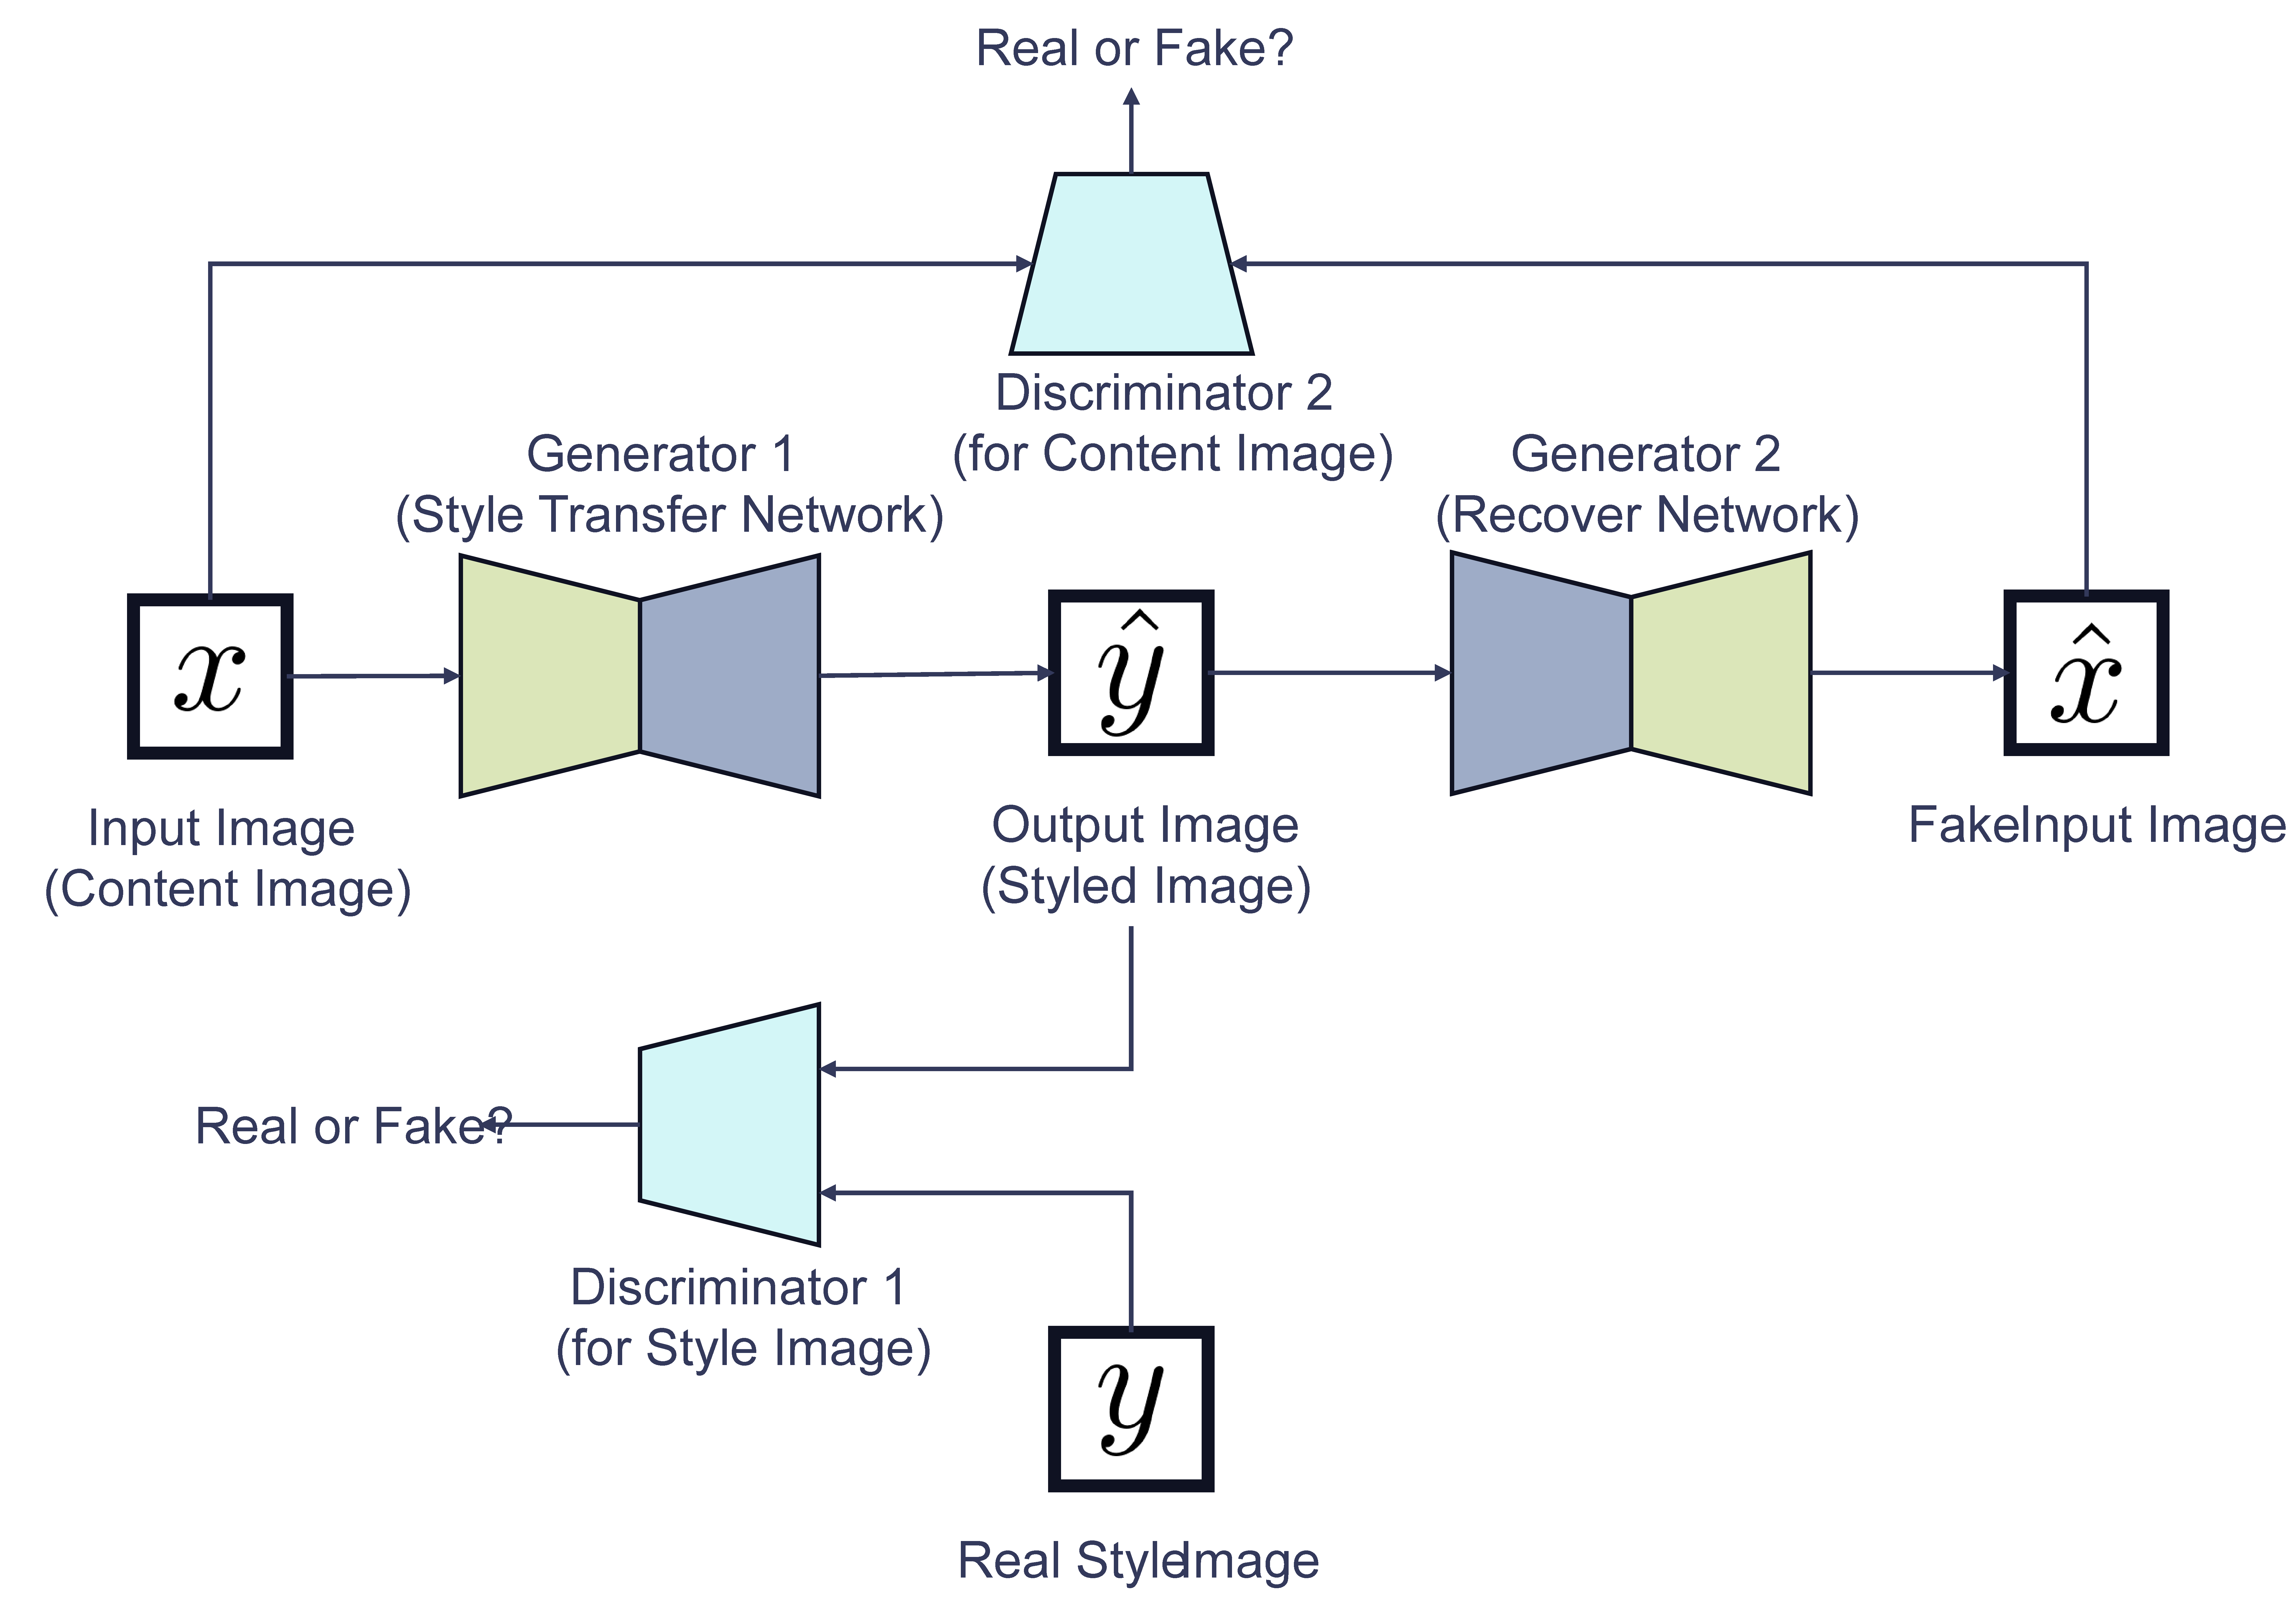
\includegraphics[width=0.95\textwidth]{fig/Figure_6_Workflow_of_CycleGAN_[38].pdf}
    %% Use \caption command for figure caption and label.
    \caption{Workflow of CycleGAN \citep{37zhu2017unpaired}}\label{fig7_Zhu}
\end{figure}

However, GANs face several issues and drawbacks when applied to real-time style transfer. Firstly, training GANs is often challenging and can be unstable, leading to problems such as mode collapse. Secondly, the loss function of GAN models does not include hyperparameters like $\alpha$ and $\beta$ from Gatys et al.’s\citep{02gatys2016image} loss function, making it difficult to control the similarity between the generated image and the content or style images. Therefore, precise control in style transfer tasks is challenging. While GANs can be used for style transfer tasks, they are not specifically designed for these tasks.

Zhu et al.\citep{37zhu2017unpaired} modified GANs\citep{38goodfellow2014generative} to better adapt to real-time style transfer tasks. In their work\citep{37zhu2017unpaired}, they proposed CycleGAN, which achieves unsupervised Per Model Per Style style transfer. CycleGAN's uniqueness lies in its introduction of "cycle consistency loss," which ensures bidirectional transformations by simultaneously training two generators and two discriminators, thus preserving information through conversions from one domain to another and back. Similar to GANs, CycleGAN\citep{37zhu2017unpaired}'s generator maps images from one domain to another, while the discriminator tries to distinguish between generated and real images (Figure \ref{fig7_Zhu}).



One of the advantages of CycleGAN is its ability to handle unpaired data, enabling unsupervised learning. This method can learn how to perform cross-domain image translation without requiring explicit pairings for each sample during training. However, CycleGAN also has some notable drawbacks in the field of style transfer. The images it generates can sometimes appear blurrier or distorted than real images. Additionally, improper selection of hyperparameters may reduce the stability of the training process or result in poor image quality.

StyleGAN\citep{19karras2019style} is another outstanding achievement in using GANs for style transfer, particularly known for its portrait editing capabilities, which can generate portraits with specific features and high realism. StyleGAN controls various details and the overall style of the generated image by adjusting the "style" parameters in the input latent space. The core innovation of StyleGAN is the introduction of a new style transfer mechanism, which allows for the separate control of image content and style at different levels, thereby improving the diversity and controllability of generated images while maintaining image quality. The advantages of StyleGAN include its ability to generate high-resolution, high-quality images and provide powerful image editing capabilities through style control. It performs exceptionally well in generating faces and other complex images. However, the training process is resource-intensive and time-consuming, requiring significant computational resources. Additionally, the generated images may sometimes contain unpredictable artifacts, necessitating further optimization to improve stability and reliability.

Men et al.\citep{46Men_2022_CVPR} focused on portrait style transfer, aiming to transform portrait photographs into anime-style avatars. They observed that when using CycleGAN for style transfer involving significant geometric deformations, it is challenging to generate high-quality transfer results while preserving the correct structure. To address this issue, the authors proposed an unsupervised cartoon image generation method based on a Gated Cycle Mapping Network (GCMN). The core of this approach is the introduction of a Gated Style Encoder (Egs), which generates category-specific style codes through domain and group-specific style layers and injects these codes into the generator to achieve precise style control.

Traditional CycleGAN models enforce bidirectional mapping, requiring multiple generators, which perform poorly when dealing with complex geometric structural changes, especially in the conversion from portraits to anime, where high-quality outcomes cannot be assured. To mitigate this limitation, Men et al. designed a gated style encoder that combines gated mapping units (GMUs) with domain-specific and group-specific layers to generate category-specific style codes, thereby achieving precise control over the transformation process. The domain-specific layers distinguish whether the image originates from the photo domain or the cartoon domain, while the group-specific layers further differentiate between portraits and scenes, ensuring the rationality and accuracy of the style transfer. Additionally, the authors introduced an Adaptive Instance Normalization (AdaIN) mechanism to inject the style codes into the generator via a multi-layer perceptron (MLP), dynamically modulating the stylistic expression within the generated results.

In contrast to traditional multi-generator or multi-encoder methods, the Gated Cycle Mapping Network requires only a single generator to handle image translation tasks in all directions, significantly simplifying the model architecture. Experimental results demonstrated that the gated style encoder not only enhanced the quality of the generated cartoon images but also allowed for flexible migration according to user-specified style requirements, thus achieving higher controllability. With these improvements, the authors' model surpassed existing state-of-the-art methods in terms of visual effects and style control and also exhibited superior performance in video synthesis tasks.Per Model Per Style transfer can mitigate the primary drawbacks of long transfer time and low efficiency of pixel-iteration-based style transfer by shifting the time required for the transfer phase to the training phase. However, the trade-off is that it can only transfer a specific, single style. If multiple styles are to be transferred using this method, corresponding network training is required for each style, resulting in a large number of parameters. In such cases, the large number of parameters makes it difficult to deploy on devices with limited resources (e.g., smartwatches), thus necessitating a balance between the number of styles and the performance constraints.

\subsubsection{Per Model Per Style}

Although the Per Model Per Style methods addressed the issue of real-time stylization and improved the efficiency of style transfer, each model can only correspond to a specific style. Transferring to a new style requires significant time for training a new model, and it is challenging to apply these models to the devices with limited resources. To address this, the networks capable of transferring multiple styles while maintaining the ability to perform fast transfers, known as Per Model Multi Style networks, are developed. One of the main approaches to achieving multi-style transfer is to bind a specific style to a small portion of the network parameters to reduce redundant parameters and combine this with the addition of necessary parameters that reflect style differences in the networks.

Dumoulin et al.\citep{39dumoulin2016learned} were the first to bind specific styles to parameters within the network, thereby achieving Per Model Multi Style transfer. In reducing redundant parameters, they noted that certain parts of the computation in the transfer of different styles are similar or identical, as many artistic styles with different names share similar or identical brushstrokes (for example, Impressionist paintings have similar brushstrokes, differing mainly in the colors used). It seems wasteful to treat these paintings with similar brushstrokes as entirely different styles. Traditional one-to-one style transfer models overlooked this, leading to unnecessary time wastage during the training phase when transferring to a new style.
In their experiments, Dumoulin et al.\citep{39dumoulin2016learned} found that scaling or transforming the normalized parameters is sufficient to adapt to a particular style. For a convolutional neural network, this finding implies that the parameters of all convolutional kernels can be adjusted to facilitate the transfer of different styles. Specifically, style transfer can be achieved by simply adjusting certain parameters of the convolutional kernels after normalization. In implementation, Dumoulin et al.\citep{39dumoulin2016learned} built upon the method of Ulyanov et al. \citep{23ulyanov2016texture}, applying an affine transformation after instance normalization to complete the transfer of different styles. This process is referred to as Conditional Instance Normalization (CIN), which can be represented by the following formula:

\begin{equation}
    \label{IN}
    \text{CIN}\left(\mathcal{F}(I_c,s)\right) = \gamma^s\left(\frac{\mathcal{F}(I_c)-\mu(\mathcal{F}(I_c))}{\sigma(\mathcal{F}(I_c))}\right)+\beta^s
\end{equation}
The input to the formula consists of the content image $I_c$ and the style index $s$, with $F(x)$ representing the feature map of image x, and $\mu(x)$ and $\sigma(x)$ representing the mean and standard deviation of the image, respectively. This method achieved the transfer of different styles by scaling or transforming the parameters $\gamma^s$ and $\beta^s$, meaning that each style s can be realized by adjusting the parameters of the affine transformation.

The advantage of this approach is that by using affine transformations on parameters of similar styles, Dumoulin et al. were able to reduce redundant parameters, significantly lowering the number of required parameters compared to Per Model Per Style methods when generating the same number of styles. However, when dealing with images with significant style differences, it is still necessary to retrain the network to obtain the corresponding style parameters and adjustment methods. Therefore, as the number of transferable styles increases, the network parameters in this method also increase.

Chen et al.\citep{40chen2017stylebank} achieved parameter simplification through a different method. Unlike Dumoulin et al.\citep{39dumoulin2016learned}, who used similar parameters to represent similar styles, Chen et al. \citep{40chen2017stylebank} considered content image processing, proposing that the parts of the network that process content information could be the same. This led to the concept of decoupling the content processing module and the style processing module within the network. By using this decoupling approach, with independent network modules learning the content and style information of an image, the network becomes more flexible in handling style transfer tasks. This method employs mid-level convolutional filters (referred to as the "StyleBank" layer in\citep{40chen2017stylebank}, as shown in Figure \ref{fig8_Chen}) specifically designed to learn different styles. The "StyleBank" layer contains multiple sets of parameters, with each set associated with a specific style.

\begin{figure}[!htbp]%% placement specifier
    %% Use \includegraphics command to insert graphic files. Place graphics files in 
    %% working directory.
    \centering%% For centre alignment of image.
    \includegraphics[width=0.95\textwidth]{fig/Figure_7_Network_Architecture_of_Chen_et_al_[41].pdf}
    %% Use \caption command for figure caption and label.
    \caption{Network Architecture of Chen et al.\citep{40chen2017stylebank}}\label{fig8_Chen}
\end{figure}

The other parts of the network, aside from the "StyleBank" layer, are used to learn content information. Since the content processing module handles different styles in the same way, different styled images can use the same content processing module, thereby improving the network's efficiency in processing various styles. When implementing multi-style transfer, only incremental training is needed. Specifically, when a new style needs to be added, the part of the network responsible for learning content information can be fixed, and only the "StyleBank" layer for the new style is trained. This approach allows the network to effectively learn new styles without affecting the existing learned ones. In the StyleBank, one or more sets of convolutional kernels represent a specific style. By placing different sets of convolutional kernels into the neural network, it can perform style transfers for different styles, providing good scalability.

Although this approach allows a single network to transfer multiple styles and optimizes the number of parameters in the network, challenges still remain. In terms of parameters, if the method attempts to transfer multiple styles, the number of parameters will gradually increase with the number of transferable styles, making it impossible for this approach to handle arbitrary style transfers. Regarding the quality of generated images, due to the partial parameter sharing, the transfer quality might not reach the excellent results of style transfer methods based on model iteration.

\subsection{Arbitrary and Real-Time Style Transfer}

The development of style transfer can be summarized in a single phrase: a trade-off between the number of styles, the quality of the transfer, the transfer time, and the resources required. However, in practical applications, users may demand both diverse style transfer and fast processing speeds. Consequently, methods that can perform arbitrary style transfer with high quality and efficiency have emerged.

Currently, mainstream methods for achieving arbitrary and real-time style transfer can be divided into three categories based on whether they use other auxiliary technologies:
\begin{enumerate}
    \item Using image spatial features or parameter matching for style transfer.
    \item Utilizing technologies such as GANs\citep{38goodfellow2014generative}, attention mechanisms, diffusion models, pre-trained large models, and others as auxiliary tools.
    \item Focusing on in-depth research into style transfer, by exploring new processes and network structures to achieve arbitrary and real-time style transfer tasks.
\end{enumerate}

Given the abundance of GAN-based methods, they are separated from the second category. Based on the above descriptions, this section will introduce the achievements in arbitrary and real-time style transfer across the following five categories:

\begin{enumerate}
    \item Style transfer based on spatial features or parameter matching.
    \item Arbitrary and real-time style transfer based on GANs\citep{38goodfellow2014generative}.
    \item Arbitrary and real-time style transfer based on attention mechanism.
    \item Arbitrary and real-time style transfer based on pretrained models.
    \item Arbitrary and real-time style transfer using self-built networks.
\end{enumerate}

The method of style transfer based on spatial features or parameter matching emerged earlier and, although the quality of the transfer effects is not ideal, it serves as an introduction to the pioneers of arbitrary and real-time style transfer. The development of the latter three categories has progressed in parallel, and the latest advancements in the field of style transfer can generally be classified into these three categories.

\subsubsection{Style Transfer Based on Spatial Features or Parameter Matching}

The style transfer methods based on spatial features or parameter matching focus on the features in the spatial domain of images, attempting to achieve arbitrary style transfer by adjusting the spatial feature parameters or matching corresponding regions between the content image and the style image.

The first work to achieve arbitrary and simultaneous style transfer was proposed by Huang et al. in 2017\citep{04huang2017arbitrary}. Inspired by the CIN method\citep{39dumoulin2016learned}, Huang et al. introduced the Adaptive Instance Normalization layer (AdaIN). This layer is used to match the variance and mean of content features with the mean and variance of style features, thereby achieving arbitrary style transfer through this matching of variance and mean. The formula for AdaIN can be described as follows:

\begin{equation}
    \label{AdaIN_equation}
    \text{AdaIN}(\mathcal{F}(I_c),\mathcal{F}(I_s))=\sigma(\mathcal{F}(I_s))\left(\frac{\mathcal{F}(I_c)-\mu(\mathcal{F}(I_c))}{\sigma(\mathcal{F}(I_c))}\right)+\mu(\mathcal{F}(I_s))
\end{equation}

Unlike the method in \citep{39dumoulin2016learned}, the encoder in Huang et al.'s style transfer network is fixed, containing the first few layers of a pre-trained VGG network. The overall structure of their network is shown in Figure 8.

\begin{figure}[!htbp]%% placement specifier
    %% Use \includegraphics command to insert graphic files. Place graphics files in 
    %% working directory.
    \centering%% For centre alignment of image.
    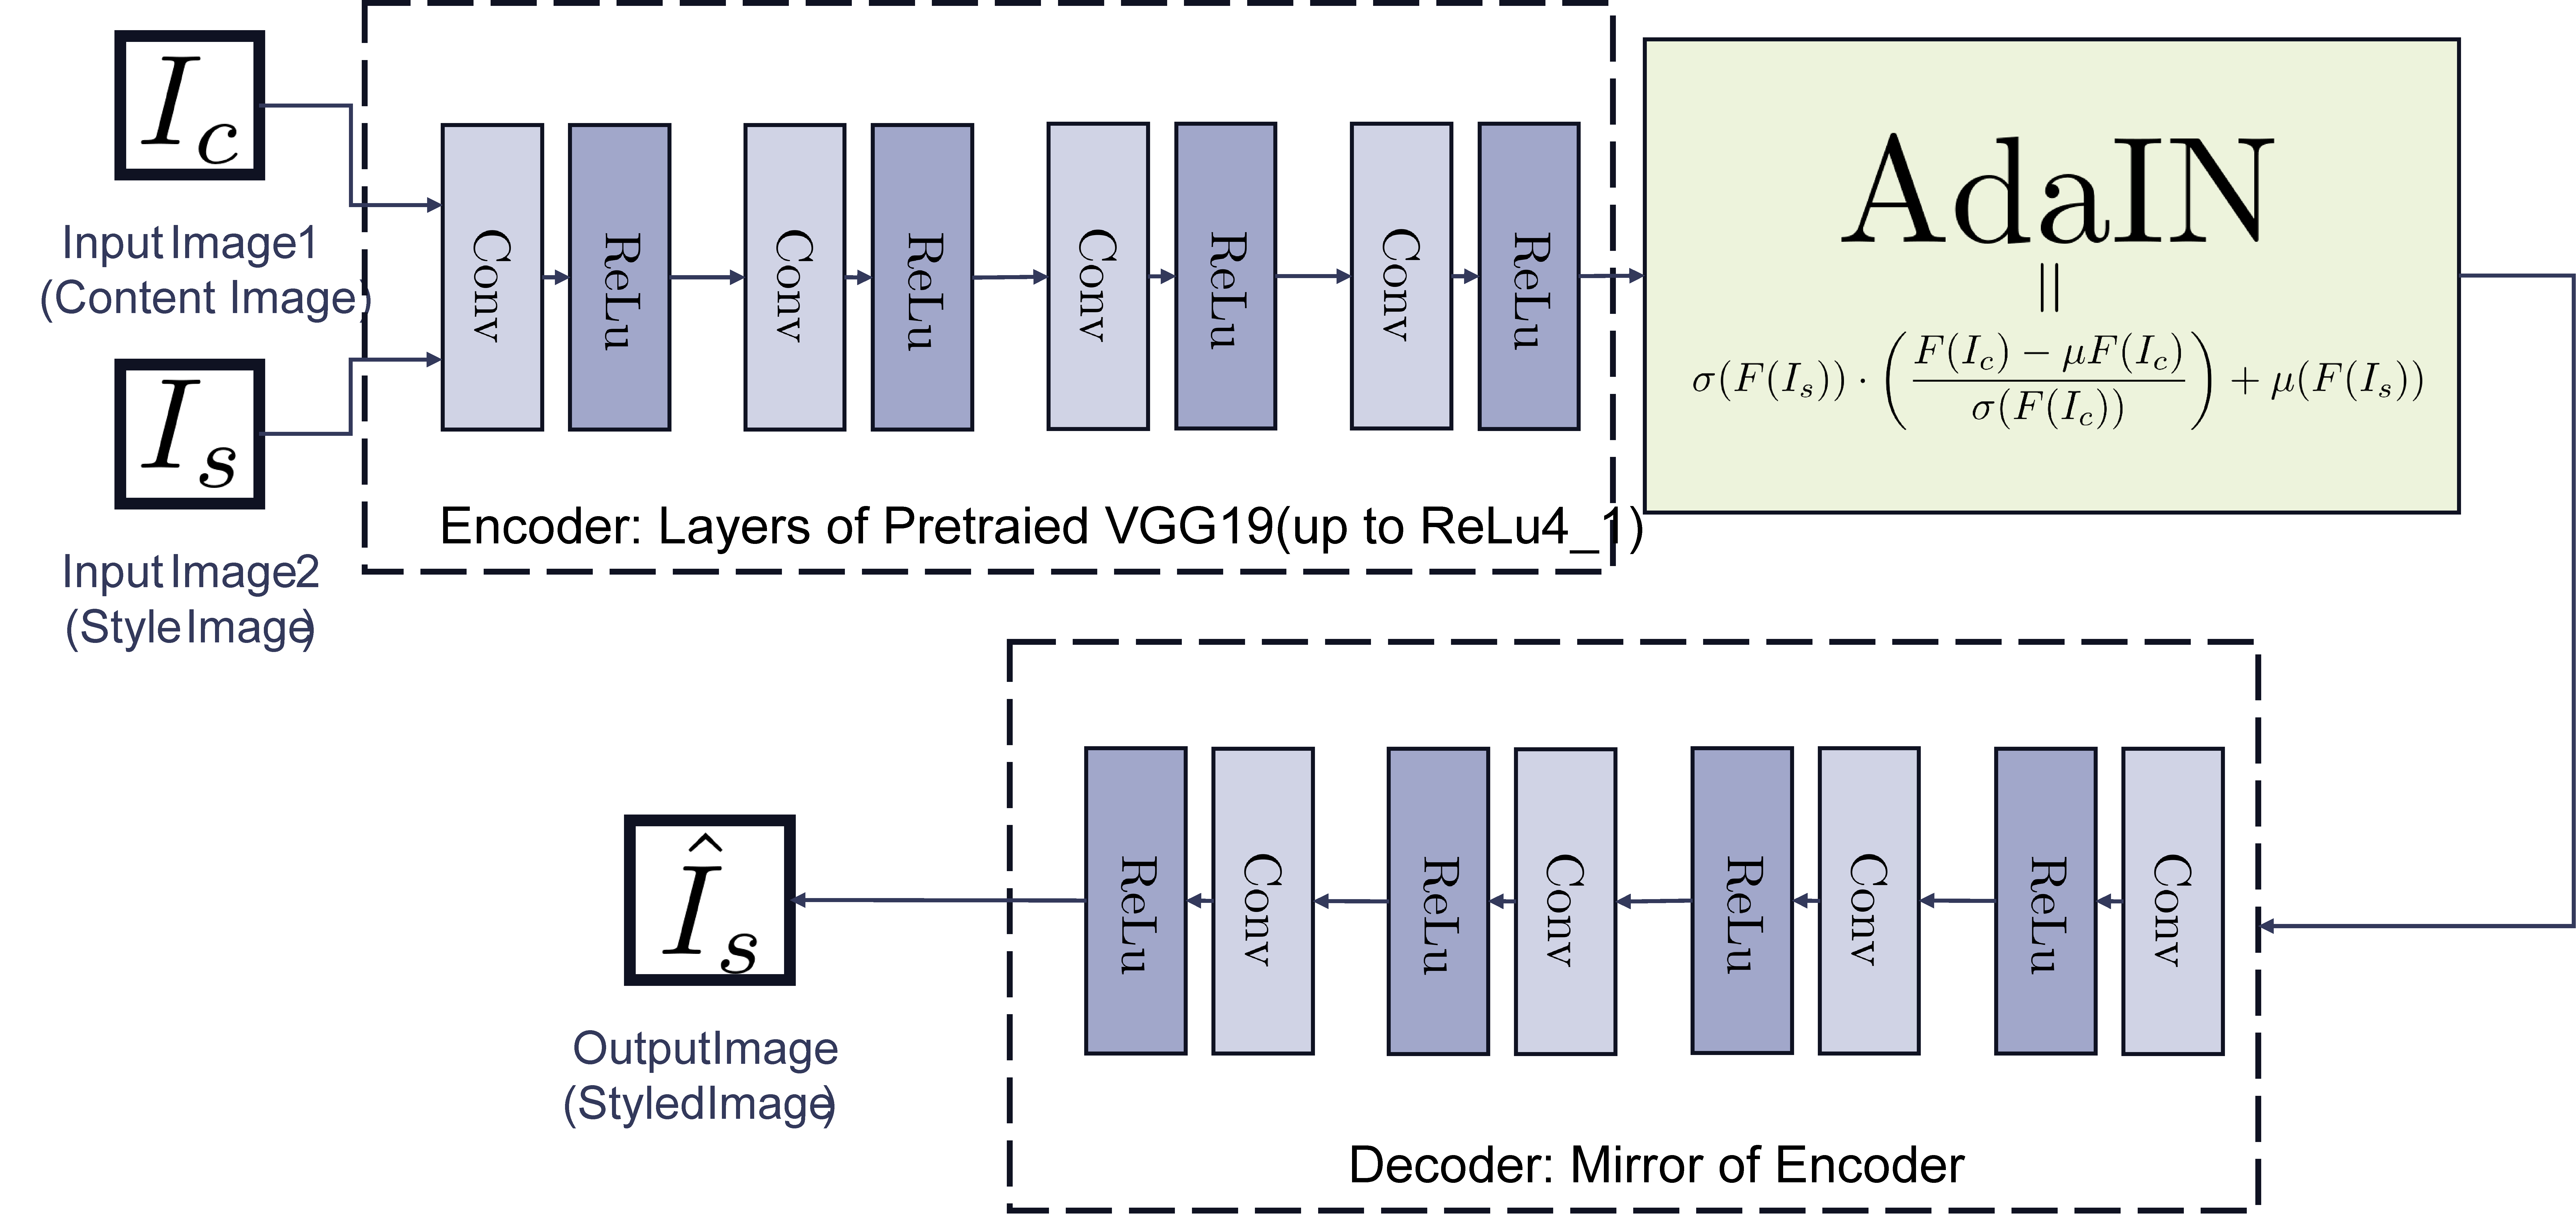
\includegraphics[width=0.95\textwidth]{fig/Figure_8_Network_Architecture_of_Huang_et_al_[4].pdf}
    %% Use \caption command for figure caption and label.
    \caption{Network Architecture of Huang et al.\citep{04huang2017arbitrary}}\label{fig8_Chen}
\end{figure}

Considering the common issues in style transfer when using normalization techniques as in previous works \citep{04huang2017arbitrary,39dumoulin2016learned}, Jing et al.\citep{41jing2020dynamic} modified AdaIN\citep{04huang2017arbitrary} and proposed the Dynamic Instance Normalization layer (DIN). The main advantage of DIN is that it allows for arbitrary style transfer by aligning the mean and variance (the simplest statistical data) between content and style features, without the need for manually defining a formula for calculating affine parameters. Instead, it introduces a more general dynamic convolution transformation, where the parameters adaptively change according to different styles in a learnable manner, thereby more accurately aligning the complex statistical data of real style features. Given a pair of content image $I_c$ and style image $I_s$ as inputs, the proposed DIN layer can be represented by the following formula:

\begin{equation}
    \begin{aligned}
        \text{DIN}(\mathcal{F}_c,\mathcal{F}_s) &= f[\mathcal{F}_s,\text{IN}(\mathcal{F}_c)],\\
        \text{IN}(\mathcal{F}_c) &= \frac{\mathcal{F}_c-\mu(\mathcal{F}_c)}{\sigma(\mathcal{F}_c)}
    \end{aligned}
\end{equation}
where $\mathcal{F}_c$ and $\mathcal{F}_s$ are the feature representations of $\mathcal{I}_c$ and $\mathcal{I}_s$, respectively, and $f$ is the dynamic convolution operation\citep{42jia2016dynamic}. Unlike standard convolution, where weights and biases are model parameters, the weights and biases in the dynamic convolution $f$ within DIN are dynamically generated by encoding different input style images. This dynamic adjustment mechanism makes DIN more flexible and precise in capturing and applying fine style features, thereby enriching the expression of style details while preserving the content structure.

The work by Chen et al.\citep{43chen2016fast} is another early effort in arbitrary style transfer called Style Swap. Unlike the methods\citep{04huang2017arbitrary,39dumoulin2016learned,41jing2020dynamic} that use image spatial feature parameter matching for style transfer, this approach focuses on the differences between the content image and the style image. The method first divides the images into multiple patches and then exchanges the most similar feature patches between the content image and the style image to achieve real-time and arbitrary style transfer. The specific steps of Step Swap can be list as follows: 
\begin{enumerate}
    \item  Extract a set of image patches from the content feature map and the style feature map, denoted as the content feature patch set$\{\phi_i(C)\}_{i\in n_c}$ and the style feature patch set $\{\phi_i(S)\}_{j\in n_s}$, where $n_c$ and $n_s$ represent the number of content feature patches and style feature patches, respectively. These patches should be sampled from all feature maps and should have sufficient overlap;
    \item  For each content feature patch, determine the closest matching style feature patch based on the normalized cross-correlation metric (Equation \ref{chen_normalized_cross-correlation measure});
    \item Swap each content feature patch $\phi_i(C)$ with its closest matching style image patch $\phi^{ss}(C,S)$;
    \item   For overlapping areas, if different values are obtained in step 3, average them.
    \begin{equation}
        \begin{aligned}
            \label{chen_normalized_cross-correlation measure}
            \phi_{i}^{s s}(C, S):=\underset{\phi_{j}(S), j=1, \ldots, n_{s}}{\operatorname{argmax}} \frac{\left\langle\phi_{i}(C), \phi_{j}(S)\right\rangle}{\left\|\phi_{i}(C)\right\| \cdot\left\|\phi_{j}(S)\right\|}
        \end{aligned}
    \end{equation}
\end{enumerate}

Through the above method, the stylized feature map can be obtained. By upsampling and reconstructing this stylized feature map, the final stylized image can be generated. Although this method achieves arbitrary and real-time style transfer with better image quality than the previously mentioned methods based on spatial feature parameter matching\citep{04huang2017arbitrary,39dumoulin2016learned,41jing2020dynamic}, it is less efficient in terms of time and resource consumption compared to those methods. Additionally, since the method uses image patches as the unit for style transfer, it overlooks global style information and lacks accuracy in measuring the similarity between adjacent image patches.

\subsubsection{GAN-Based Arbitrary and Real-Time Style Transfer}

Given the advantages of GANs, such as powerful unsupervised learning capabilities, feature learning abilities, and data generalization, researchers have considered further adjusting GANs to enhance their style transfer capabilities as style transfer advances to the arbitrary and real-time stage.

To the best of our knowledge, Xu et al.\citep{44xu2021drb} were the first to use GANs to achieve arbitrary and real-time style transfer. They proposed the Dynamic Residual Block Generative Adversarial Network (DRB-GAN) for style transfer. The concept of Dynamic Residual Blocks (DRBs) was inspired by DIN and StyleGAN, modeling the "style code" as shared parameters of dynamic convolution and AdaINs within the dynamic residual blocks. Multiple DRBs were designed at the bottleneck of the style transfer network. Each DRB consists of a convolutional layer, a dynamic convolutional layer, a ReLU layer, an AdaIN layer, and an instance normalization layer with residual connections. This structure enables the adjustment of the shared parameters of dynamic convolution and adaptively modifies the affine parameters of AdaINs, ensuring statistical matching between the bottleneck feature spaces of the content and style images. The use of dynamic residual blocks is motivated by their ability to provide flexible parameter adjustments, which better achieve statistical feature matching between style and content. This design allows the network to effectively blend various style features while maintaining the basic structure of the content image.

Yang et al.\citep{45yang2022pastiche}, building on StyleGAN\citep{19karras2019style}, observed that StyleGAN is only capable of fast transfer for specific styles but cannot perform real-time transfer of arbitrary styles or generate truly artistic portraits. To address these challenges, Yang et al. proposed DualStyleGAN to achieve sample-based portrait style transfer. DualStyleGAN retains an internal style path from StyleGAN to control the style of the original domain while adding an external style path to model and control the style of the target extended domain. Additionally, the external style path inherits StyleGAN's layered architecture, modulating structural style in the coarse resolution layers and color style in the fine resolution layers, enabling flexible multi-level style operations. Although DualStyleGAN can achieve flexible portrait style transfer, the network often misidentifies other objects in the background of the content image as faces, resulting in the generation of undesired patterns.

Wu et al.\citep{47wu2023preserving} approached the style transfer problem from a different angle. They argued that even within the same artist's body of work, there can be a wide variety of artistic styles, so homogenizing different styles from the same artist is not a rigorous approach. Furthermore, existing methods often lack generalization for unseen artists. To address these challenges, Wu et al. proposed a Double-Style Transferring Module (DSTM). This module extracts different artistic styles from various artworks and retains the intrinsic diversity among different artworks by the same artist. Recognizing that learning style from a single artwork could lead to overfitting and the introduction of style image structural features, Wu et al. further introduced an Edge Enhancing Module (EEM). This module extracts edge information from multi-scale and multi-level features to enhance structural consistency. The advantage of this approach is that it can result in stylized artworks where the content features of the content image are well-preserved, with minimal intrusion of content features from the style image.

\subsubsection{Arbitrary and Real-Time Style Transfer Based on Attention Mechanisms}

The utilization of attention mechanisms in deep neural networks has gradually become a common choice for style transfer tasks. Previous achievements in style transfer often placed more emphasis on the overall style of the image, neglecting the correspondence of local styles. By incorporating attention mechanisms, which are adept at capturing the spatial layout and semantic relationships within images, style transfer models can effectively identify key regions within an image and apply style features precisely to these areas. This enables the models to achieve a balance between global and local styles to a certain extent.

Furthermore, attention mechanisms permit the exchange of features across different images, which is particularly critical for achieving nuanced style transfer effects. This capability enhances the model's ability to selectively focus on relevant parts of the input data, thereby improving the quality and coherence of the transferred style across the entire image.

Liu et al.\citep{48liu2021adaattn} sought to leverage the characteristics of the aforementioned attention mechanisms to enhance the local quality within the stylized results. They observed that existing solutions either focus solely on integrating deep style features into deep content features without considering feature distributions or adaptively normalize deep content features based on style to match global statistics\citep{04huang2017arbitrary,39dumoulin2016learned,41jing2020dynamic}. While effective, these methods concentrate only on deep and global image features, overlooking shallow and local features, which can lead to local distortions. To address this issue, Liu et al. proposed a novel attention and normalization module called Adaptive Attention Normalization (AdaAttN), which performs attention normalization adaptively on a per-pixel basis. The process of AdaAttN involves three steps: 1. Computing attention maps with content and style features from shallow to deep layers; 2. Calculating weighted mean and standard deviation maps of the style features; 3. Adaptively normalizing content features to align per-pixel feature distributions. The output of AdaAttN is then processed by a decoder to complete the style transfer. This method utilizes attention mechanisms to consider local information matching, achieving more detailed and personalized style transformations, thus enhancing the local visual quality of the image.

In contrast to Liu et al.’s approach, which addresses the neglect of local features, Deng et al.\citep{49deng2022stytr2} argue that CNNs have limited receptive fields and can only perceive local information, making it challenging to extract and maintain global information from the input image. To address this issue, Deng et al.\citep{49deng2022stytr2} proposed a Transformer-based method named StyTr2 that considers the long-range dependencies of input images. StyTr2 comprises two distinct Transformer encoders that generate domain-specific sequences for content and style. After encoding, a multi-layer Transformer decoder is used to stylize the content sequence according to the style sequence. StyTr2 mitigated the content leakage issue inherent in CNN-based models, achieving better style transfer results. However, due to the large parameters of Transformers, the approach by Deng et al.\citep{49deng2022stytr2} is somewhat less efficient in terms of runtime compared to previous methods.

Li et al.\citep{50li2023compact} also noted the difficulty of CNN-based methods in capturing long-range information and, considering the high computational cost of Transformer-based methods, they attempted to balance between long-range information and a large number of parameters while partially addressing the remaining content leakage issue. To resolve the computational and leakage problems, Li et al. designed a compact Transformer named AdaFormer. This design utilizes image patch projection and positional encoding to enhance global interactions and assumes that the differences between content and style features are captured in the higher layers of the encoder. AdaFormer achieves more efficient feature extraction by sharing parameters in the initial Transformer encoding layer and then extracting content and style features through their respective encoding layers. The algorithm also employs a multi-layer Transformer decoder for feature fusion and selects style elements through dynamic weighting. Additionally, adaptive instance normalization (AdaIN)\citep{04huang2017arbitrary} is used instead of layer normalization to make the style more consistent with the content. Finally, the upsampling decoder generates diverse stylized outputs. Compared to StyTr2\citep{48liu2021adaattn}, Li et al.’s method does reduce memory usage but still requires approximately 35GB of memory\citep{50li2023compact}.

Zhang et al.\citep{51zhang2024rethink} integrated attention mechanisms into the classic Adaptive Instance Normalization (AdaIN)\citep{04huang2017arbitrary} method to improve upon it. They identified several shortcomings in current AdaIN-based\citep{04huang2017arbitrary} style transfer works, including mismatches between content and style, image artifacts, and inaccuracies in the extraction of style features during the generation of high-quality stylized images.Zhang et al.\citep{51zhang2024rethink} analyzed two main causes for these issues: (1) the use of the VGG network for feature extraction, and (2) the reliance on statistical parameter adjustments alone during instance normalization as a means of style transfer.
For the first issue, Zhang et al.\citep{51zhang2024rethink} noted that the VGG network, originally designed for image classification, tends to focus excessively on irrelevant classification information during style transfer. To resolve this, they proposed a Transformer-based style feature extractor called the Perception Encoder (PE). The PE captures long-range dependencies and high-frequency style details in the style image, thereby avoiding the limitations of the VGG network, which focuses predominantly on prominent classification features such as edges or shapes, leading to more accurate extraction of style information.

To address the second issue, they introduced Style Consistency Instance Normalization (SCIN). Unlike AdaIN, which achieves style transfer through simple alignment based on mean and variance, SCIN uses a Transformer to capture long-range, non-local dependencies within the style feature maps, providing richer style information. Additionally, the scaling and shifting parameters generated by SCIN are learned, allowing better adaptation to the distribution of different style images rather than relying solely on fixed statistical features like mean and variance. This improvement makes SCIN more flexible and accurate in aligning style and content features, reducing artifacts and enhancing the quality of stylized images.

To further improve the quality of style transfer results and increase the distinctiveness of stylized images of different styles, the paper also proposed Instance-based Contractive Learning (ICL). ICL helps the model learn the relationships between stylized images, ensuring that embeddings of images with the same content or style are closer together, while those of different styles are further apart, thereby enhancing the quality of the stylized images.

Through the implementation of these three approaches, the paper addresses the limitations of AdaIN\citep{04huang2017arbitrary}, which considers only the unification of global features, reducing artifacts and ultimately improving the quality of stylized images from both a global and local perspective.

Wang et al.\citep{52wang2023interactive} took a different approach, asserting that the textures produced by current style transfer methods are unpredictable and do not align with artistic creation logic. They emphasized the importance of interactive participation in the style transfer process. To generate predictable textures, Wang et al. proposed an Interactive Image Style Transfer Network (IIST-Net). This network produces stylized results of brushstrokes guided by doodle curves, ensuring that the style distribution of the stylized image is closer to real-world artworks. Specifically, IIST-Net consists of two encoders, an Interactive Brush-texture Generation (IBG) module, a Multilayer Style Attention (MSA) module, and a decoder. The two encoders encode content style images and brush texture images to produce multi-layer style features and fused content features, respectively. The IBG module generates controllable brush textures based on user input, while the MSA module further refines multi-layer style features and integrates them with the fused content features. Although this method partially addresses the interactivity gap in neural style transfer, it overly emphasizes texture, making it challenging to highlight content features.

Zhang et al.\citep{53zhang2023edge} recognized the importance of balancing content and style features. They noted that excessive style patterns in image stylization could obscure content details, sometimes making it difficult to distinguish objects in the image. To address the balance between content and style, Zhang et al. proposed a Transformer-based style transfer method called STT (Style Transfer via Transformers). In this method, Transformers are primarily used for encoding content and style features and for decoding. To maintain the clarity of the content structure in the stylized image, Zhang et al. designed a novel edge loss to enhance object edges in the output image. Unlike edge detection or contour extraction tasks, the content details in style transfer outputs may differ from those in the content image, especially as the background may adopt artistic patterns from the style image. Therefore, using the similarity between edge maps of the content and stylized images directly as an optimization objective could result in blurry outcomes. One of the challenges is filtering out edges not present in the content image's main structure. Zhang et al. introduced a masking operation to address this issue: edges in the stylized image's edge map that do not correspond to positions in the content image's edge map are masked out. Additionally, Zhang et al. set a threshold to exclude weak responses in the edge map to prevent potential noise. Zhang et al.’s method achieves a balance between style and content patterns in the stylized image, resulting in a better visual experience, and somewhat alleviates the content leakage problem. However, similar to other methods using Transformers, it requires more time and resources compared to arbitrary and real-time style transfer methods that do not use Transformers.

Hong et al. [54] expressed concerns about mismatched training data in style transfer. They argued that the low semantic correspondence between arbitrary content and style images causes attention mechanisms to focus on limited regions of the style image. This impedes attention-based methods from accurately capturing and expressing the entire style of the reference image, leading to discordant patterns. To overcome these limitations, Hong et al. focused on enhancing the attention mechanism and capturing the rhythm of textures in the style image. They designed a pattern repetition rate to measure how well different style features represent the entire style image. By selecting the style with the highest pattern repetition rate as the primary style for stylization, they effectively avoided generating discordant patterns in the output image. 

Zhu et al.\citep{55zhu2023all}, almost simultaneously with Hong et al.\citep{54hong2023aespa}, observed the issue of repeated style features in style images, but achieved the selection of primary style features through a different approach than Hong\citep{54hong2023aespa}. Zhu et al.'s solution is a novel All-to-Key (A2K) mechanism, which matches each query with stable keys. A2K consists of two main components. First, the distributed attention mechanism (Figure \ref{fig9_Zhu}). To address the issues of All-to-All attention, distributed attention initially learns distributed key points to describe local regions of style features. Each query of content features is then matched with these representative key points. Since the matched key points represent regional styles rather than isolated locations, distributed attention can tolerate matching errors better. Moreover, because these key points represent several local regions, the matching performance of distributed attention is more stable across different query locations. Second, the progressive attention mechanism. Unlike traditional All-to-All attention, which directly focuses on specific locations, the progressive attention mechanism initially attends to coarse-grained regions and then gradually focuses on fine-grained positions. This approach helps match style patterns at a larger scale, finding more similar semantics within coarse-grained style patterns. On this basis, point-to-point attention further refines fine-grained positions within coarse-grained regions. Additionally, since queries within the same local region match the same key points, the transformed features also exhibit regional stability.

\begin{figure}[!htbp]%% placement specifier
    %% Use \includegraphics command to insert graphic files. Place graphics files in 
    %% working directory.
    \centering%% For centre alignment of image.
    \includegraphics[width=0.95\textwidth]{fig/Figure_13_Zhu_et_al_’s_Distributed_Attention_[55].pdf}
    %% Use \caption command for figure caption and label.
    \caption{Zhu et al.'s Distributed Attention\citep{55zhu2023all}}\label{fig9_Zhu}
\end{figure}

Through the innovative attention mechanisms described, Zhu et al. similarly improved upon the issues caused by full attention mechanisms, avoiding discordant patterns in the generated images. However, their exploration in enhancing style expressiveness\citep{55zhu2023all} remains somewhat similar to previous works in terms of expressiveness.

\subsubsection{Arbitrary and Real-Time Style Transfer Based on Pretrained Models}

Pretrained models are deep learning models that have been trained on extensive datasets, possessing broad knowledge and substantial learning capability. These models can be fine-tuned for specific tasks to improve performance and efficiency. Recently, numerous studies have sought to leverage large models to assist in style transfer tasks. Here we focus on the achievements in style transfer using large models.

Utilizing the CLIPc\citep{56radford2021learning} large model for style transfer assistance has become a current research hotspot. Kwon et al.\citep{57kwon2022clipstyler} observed that in many practical situations, users may lack reference style images but still wish to experience the results of style transfer. To address such applications, Kwon proposed a new framework aimed at transferring the semantic style of target text to content images using a pretrained CLIP model. During the process of obtaining semantically transformed images solely through CLIP supervision, Kwon found that traditional pixel optimization methods could not reflect the desired texture. To resolve this issue, Kwon et al. introduced a CNN encoder-decoder model to capture hierarchical visual features of the content image while simultaneously adding style in the deep feature space to achieve realistic stylization results. The advantage of Kwon et al.'s method lies in achieving realistic style transfer results through changes in text conditions alone, without requiring any style images. However, due to the use of large models, this method involves longer inference time compared to other methods.

\textbf{Diffusion Models.}\quad Diffusion models are generative models that were first detailed with mathematical proofs, derivations, and runnable code by Ho et al.\citep{58ho2020denoising}. These models can generate target data samples from noise and consist of two processes: the forward process and the reverse process, where the forward process is also known as the diffusion process. The forward process is a noising process, where an image $x_t$ only depends on the previous $x_(t-1)$. This process can be viewed as a Markov process:

\begin{equation}
    q (x_ {1:T}|x_0) = \prod_ {t = 1}^ {T}q (x_t|x_ {t-1}) q (x_t|x_ {t-1}) = N (x_t, \sqrt {1-\beta_t}x_ {t-1},\beta_t I)
\end{equation} 
where$\beta_t$ is a set of predefined hyperparameters, meeting the demand of  $\beta_1<\beta_2<...<\beta_T$. The reverse process is a denoising process; if the reverse process $ q (x_ {t-1}|x_ {t})$ is obtained, an image can be progressively restored from random noise $x_T$.

Hamazaspyan and Navasardyan\citep{59hamazaspyan2023diffusion} combined diffusion models with style transfer tasks, proposing a Diffusion-Enhanced PatchMatch (DEPM) model. This model utilizes Stable Diffusion to capture high-level style features while preserving fine-grained texture details of the original image. DEPM allows for the transfer of arbitrary styles during inference without any fine-tuning or pre-training, making the process more flexible and efficient.

Zhang et al.\citep{60zhang2024artbank} considered style transfer from pretrained Stable Diffusion models\citep{61rombach2022high}. They noted that methods based on small models can preserve content structure but fail to generate highly realistic stylized images, introducing artifacts and discordant textures. Conversely, pretrained model methods can generate highly realistic stylized images but struggle to maintain content structure. To address these issues, Zhang et al. proposed ArtBank, which can generate highly realistic stylized images while preserving the content structure of the content image. Specifically, to fully exploit the knowledge within pretrained models, they designed an implicit style prompt library consisting of a set of trainable parameter matrices to learn and store knowledge from an art collection, serving as visual prompts to guide the pretrained model in generating highly realistic stylized images while maintaining content structure. During the training phase, Zhang et al. introduced a novel spatial-statistics-based self-attention module to accelerate the convergence of the implicit style prompt library. By training the implicit style prompt library, Zhang et al. effectively extracted relevant knowledge from Stable Diffusion (Ver 1.4) to accomplish style transfer. Zhang et al.'s method pioneered a new approach to style transfer, focusing on how to quickly and effectively extract the necessary knowledge from pretrained models.

Building on diffusion models, Zhang et al.\citep{62zhang2023inversion} proposed a novel approach to style transfer, focusing on learning implicit textual labels of various artistic styles as the core of style transfer. The primary concept of this method is to treat the style in artwork as a learnable textual description of a painting and to guide the Diffusion model in generating images based on style labels. In terms of implementation, Zhang et al. proposed Inversion-Based Style Transfer Method (InST) and employed it to efficiently and accurately learn image-related information. Specifically, a conditional generative model is used to learn the correspondence between images and text, thereby obtaining image embeddings. Based on these image embeddings, an attention-guided inversion module receives the embeddings and utilizes an attention mechanism to generate corresponding text embeddings. This module focuses on various features in the image embeddings, such as semantics, texture, object shape, brushstrokes, and color, ultimately resulting in the corresponding text embeddings and text labels. These text labels guide the Diffusion model in style transfer. The text labels need not be describable in natural language but are a sequence of characters or a token (token) that only the Diffusion model can interpret to describe the style. Once learned, the Diffusion model can fix the style corresponding to this label, making this method a model-based iterative approach to style transfer. The distinctive feature of this approach is its ability to alter the shape of the image during the stylization process, which was not possible with previous style transfer models.

Similarly, Namhyuk et al.\citep{63ahn2024dreamstyler} observed that style information is difficult to describe accurately in language; therefore, they considered encoding style images into the text space to provide textual constraints for Stable Diffusion. Specifically, Namhyuk et al.\citep{63ahn2024dreamstyler} combined style transfer with text-to-image generation tasks based on Stable Diffusion, proposing the DreamStyler framework. This framework is capable of extracting style information from images into the CLIP text space.
To integrate textual descriptions with Stable Diffusion, the authors proposed the concept of extended text embedding space based on Textual Inversion (TI). This idea involves dividing the time steps of the diffusion model into multiple groups, each referred to as a Chunk of Timesteps. A combination of a Chunk of Timesteps with corresponding textual descriptions is termed a TI Stage. By combining multiple TI Stages, Stable Diffusion can understand similar yet distinct style description embeddings at different time step chunks during image synthesis. This method is referred to by the authors as Multi-Stage Textual Inversion.
Additionally, Namhyuk et al.\citep{63ahn2024dreamstyler} introduced context-aware prompt enhancement, which can decouple style and contextual information from style images. After decoupling, the style information can be encoded as special text embeddings, providing more accurate style descriptors for use with Multi-Stage Textual Inversion.

Wang et al.\citep{64wang2023stylediffusion} developed a framework called StyleDiffusion, which achieves the separation of image style and content. This framework is based on the Diffusion model and uses the diffusion process to separately remove style information and content information from the image. It then utilizes a CLIP-based style disentanglement loss, coordinated with style reconstruction priors, to achieve complete disentanglement of content and style. The framework comprises three key components: a diffusion-based style removal module, a diffusion-based style transfer module, and a CLIP-based style disentanglement loss coordinated with style reconstruction priors. Experiments demonstrate that this framework can produce high-quality style transfer results and better considers the relationship between content and style compared to other methods. In contrast to previous methods, this approach completely decouples content (C) and style (S) through the diffusion model, thereby providing a more nuanced understanding of their relationship. Consequently, the style transfer results are more natural and harmonious, especially for challenging styles such as Cubism and oil painting. Wang et al.’s method achieves precise control over the style transfer process through the diffusion model and CLIP-based style disentanglement loss. By adjusting parameters, one can flexibly control the degree of style removal and the extent of content-style disentanglement, leading to more desirable style transfer outcomes. Moreover, this method has high interpretability and scalability. The introduction of the diffusion model and CLIP-based style disentanglement loss makes the style transfer process more interpretable. Additionally, this method can be applied to other image transformation or manipulation tasks, demonstrating significant scalability.

Lu et al.\citep{65lu2023specialist} attempted to address the challenge of fine-tuning a pre-trained diffusion model with a minimal number of image samples to learn any unseen style. They proposed a method called "Specialist Diffusion," which enables the learning of any unseen style by fine-tuning a pre-trained diffusion model with only a small number of images (e.g., fewer than 10). This method allows the fine-tuned diffusion model to generate high-quality images of arbitrary objects in a specified style. To achieve such low-sample fine-tuning, Lu et al. introduced a novel set of fine-tuning techniques, including custom data augmentation for text-to-image tasks, content loss to facilitate the disentanglement of content and style, and sparse updates focusing on only a few time steps.The "Specialist Diffusion" method can seamlessly integrate with existing diffusion models and other personalization techniques, achieving superior fine-tuning performance compared to state-of-the-art few-shot personalized diffusion models, particularly in learning highly complex styles. Moreover, "Specialist Diffusion" can be combined with inversion methods to further enhance performance, even achieving success with very unusual styles. However, the method does have certain limitations. Firstly, while it effectively fine-tunes with a small number of images to learn unseen styles, there may still be cases where learning is insufficient for highly specific and unusual styles. Secondly, although the method demonstrates good sample efficiency, the generated results may be suboptimal for some complex or content close to the training data distribution. Lastly, the performance of this method is constrained by the quality of the pre-trained model; if the pre-trained model is of poor quality, it may adversely affect the results of the fine-tuning. 

Chung et al.\citep{66chung2024style} aimed to address the issue of excessive inference times when using diffusion models for style transfer tasks. Although there were already training-free approaches available, previous research had not effectively applied these methods to large diffusion models such as Stable Diffusion. By reviewing existing literature, Chung et al. identified two key characteristics of using large diffusion models for image translation: first, attention maps determine the spatial layout of the generated images; second, adjusting the queries and keys in the cross-attention mechanism can influence the content of the generated images.

Based on these findings, Chung et al. proposed a strategy for style transfer without retraining the diffusion model. The core idea of this strategy is to replace the queries and keys in the self-attention maps of the content image with those derived from the style image’s self-attention maps. When implementing this core idea, Chung et al. encountered two primary issues: content disruption and color errors. To address content disruption, they introduced a “query preservation” strategy. For color errors, they employed Initial Latent Adaptive Instance Normalization (Initial Latent AdaIN) technology.

By combining these three elements, their method achieved a training-free style transfer approach based on large diffusion models. The advantage of this method lies in its ability to maintain the relationship between queries in the content image if they share similar semantics, as they will utilize similar keys after style transfer. Moreover, the high similarity between queries of the content image and keys with similar textures and semantics in the transfer results leads to a more natural and harmonious effect in the style transfer outcome.

Unlike Namhyuk et al. \citep{63ahn2024dreamstyler}, who encoded style information into the text space, Deng et al.\citep{67deng2024z} believed that using an encoder to convert style images into text features to guide the Stable Diffusion model could lead to significant losses because such textual feature descriptions are imprecise, resulting in outputs that often fail to capture the detailed style features of the images adequately. They pointed out that fundamental diffusion models can directly extract style information without textual constraints, given that the commonly used U-Net architecture in such models possesses this capability, thereby achieving the goal of avoiding dependence on text embeddings.

Based on this insight, Deng et al. proposed a dual-path denoising model based on Stable Diffusion to achieve style transfer. This model consists of two independent yet identical diffusion models, one handling content images and the other handling style images, both employing a U-Net as the core network. For ease of description, these two diffusion models are referred to as the Style Diffusion Model and the Content Diffusion Model. The Style Diffusion Model aims to reconstruct the original style image progressively through a T-step diffusion process from a noise image. Similarly, the Content Diffusion Model aims to reconstruct the content image.

When the diffusion models operate at any time step $t \in [0, T]$, the U-Net extracts content feature maps $X^c_t$ from the content diffusion path and style feature maps $X^s_t$ from the style diffusion path. These feature maps are then combined through a cross-attention mechanism to generate a stylized latent feature map $\hat f_c$. Subsequently, these latent feature maps pass through a reverse diffusion process to produce the final stylized image. Compared to traditional methods that compute style features based on Gram matrices, this approach can better preserve the structure and details of the content image.

The integration mechanism described herein is termed "Cross-Attention Reconstruction," with the central idea being to treat different pixels within the content image as Queries, which are correlated with the features (Keys) of the style image. Given that the relevance between content pixels and style information may vary, these differences can influence the effect of style transfer. Some content pixels might contribute disproportionately to the style information, leading to regions within the stylized result that appear unnatural or compromise the fidelity of the content. Therefore, the authors propose applying a weighted suppression to these less relevant content pixels to diminish their impact on the stylized latent feature map $\hat f_c$.

However, due to the properties of the Softmax function, pixels with lower relevance (i.e., those with smaller  $QK^T$ values) might end up receiving relatively larger attention weights after the Softmax operation, leading to suboptimal style transfer outcomes. To address this issue, we introduce a reweighted cross-attention mechanism that incorporates an adjustable weighting parameter $\lambda$ into the Softmax function, dynamically modulating the attention weights of different pixels. This approach not only mitigates the influence of low-relevance pixels but also effectively enhances the representation of pixels strongly correlated with the style image.

Based on the aforementioned methodology, Deng et al. have realized a novel style transfer method grounded in diffusion models that does not require textual embeddings. This method ensures that the stylized results retain the details of the content while accurately reflecting the stylistic characteristics.

\subsubsection{Arbitrary and Real-Time Style Transfer Based on Self-Built Networks}

\textbf{Frequency Domain-Based Approach.}\quad Frequency domain processing holds significant importance in the field of computer imaging. It involves transforming images from the spatial domain to the frequency domain to analyze and modify the frequency characteristics of images. This approach is instrumental in achieving various critical tasks such as filtering, compression, and feature extraction. Frequency domain processing effectively reduces noise, enhances image quality, detects edges and texture details, and provides powerful tools for applications such as image compression and recognition, offering a wealth of technical means for research and application in the field of image processing.

The approach proposed by Li et al.\citep{03li2023frequency} differs from most previous methods \citep{04huang2017arbitrary,40chen2017stylebank,50li2023compact,55zhu2023all,68zitnick2014adopting,69zhang2017style} that focus on the spatial domain, as it considers the content and style features of images from the frequency domain perspective. Li et al. argue that effective disentanglement of content and style is crucial for synthesizing images in arbitrary styles. They note that existing methods tend to focus on disentangling content and style feature representations in the spatial domain, where content and style features are inherently entangled. This entanglement leads to issues such as local distortions, weaker generalization capability, and inflexibility in previous methods. Li et al.’s approach is based on the observation that images or feature maps can be transformed into the frequency domain, where the low-frequency components describe smooth variations, and the high-frequency components are associated with rapid changes\citep{70chen2019drop}. This characteristic is referred to by them as the Frequency Separable Property (FSP).

Based on the Frequency Separable Property, Li et al. proposed the FreMixer module, which is capable of disentangling and re-entangling the frequency spectra of content and style components in the frequency domain. Since content and style components exhibit distinct frequency domain characteristics (such as frequency bands and patterns), FreMixer effectively decomposes these two components. The procedure is as follows: Firstly, a two-dimensional fast Fourier transform (2-D FFT) is performed along the spatial dimensions to convert spatial feature maps into the frequency domain; next, frequency kernels learned through the network are introduced, serving a role similar to that of global depth convolutional layers, to disentangle the content and style frequency parts in the spectral map; thirdly, after disentangling the content and style frequency patterns, the two frequency spectra are recombined through element-wise addition; and finally, the frequency spectra are converted back into spatial domain stylized features using a two-dimensional inverse fast Fourier transform (2-D IFFT). By following these steps, content and style can be separated in the frequency domain and then recombined in the spatial domain to achieve image style transfer. Li et al.'s work\citep{03li2023frequency}, starting from the frequency domain, achieves the decoupling of style and content features, pointing out a new direction for neural style transfer.

Kwon et al.\citep{71kwon2024aesfa}, although approaching the problem from a different perspective than Li et al.\citep{03li2023frequency}, reached similar conclusions. Kwon posits that current style transfer methods struggle to effectively transfer aesthetically pleasing artistic information and face high computational costs and poor feature disentanglement due to the use of pre-trained models. To address this, they propose a lightweight yet effective model called the Aesthetic Feature-Aware (AesFA) model. Similar to Li et al.\citep{03li2023frequency}, Kwon et al.'s primary idea is also to decompose images through their frequency to better separate aesthetic styles from reference images. During training, the entire model is trained end-to-end to completely eliminate pre-trained models during inference. Additionally, to enhance the network's ability to extract more distinctive representations and further improve style transfer quality, Kwon et al. introduce a new loss function: the Aesthetic Feature Contrast Loss. This method generates stylized images with superior features, and AesFA also shows reduced time consumption when transferring high-resolution images, demonstrating good style transfer performance.

\textbf{Constructing Novel Feature Extractors.} \quad Wang et al.\citep{72wang2023microast} address the efficiency of style transfer algorithms by noting that existing arbitrary style transfer methods struggle or are unable to handle ultra-high-resolution images (e.g., 4K), which significantly hinders their further application. They reconsidered the entire style transfer process and identified that the slow transfer speeds are primarily due to the widespread use of VGG\citep{25simonyan2014very} as a feature extractor in previous neural style transfer methods. This is because the fully connected layers of large pre-trained deep convolutional neural networks (DCNNs) require substantial computational resources.

To develop a style transfer model that can efficiently perform tasks on high-resolution images, Wang et al. completely abandoned the traditional use of VGG\citep{25simonyan2014very} as the content and style feature extractor. Instead, they designed an entirely new feature extractor, naming the overall network model MicroAST. Additionally, Wang et al. proposed a new loss function called "Style Signal Contrastive Loss" to assist MicroAST in style transfer tasks. MicroAST consists of two main components: a micro encoder and a micro decoder. The micro encoder is further divided into a micro content encoder and a micro style encoder, which share the same structure, including one standard stride-1 convolutional layer, two stride-2 depthwise separable convolution (DS Conv) layers, and two stride-1 residual blocks (ResBlocks). The structure of the micro decoder is nearly symmetrical to that of the micro encoder. By discarding the VGG\citep{25simonyan2014very} feature extractor, Wang et al. significantly reduced the time and memory required for high-resolution style transfer while achieving satisfactory style transfer results.

It is worth noting that the study by Kwon et al.\citep{71kwon2024aesfa} also discarded the traditional VGG\citep{25simonyan2014very} feature extractor to achieve higher speed and lower memory usage. However, the core of that study lies in the other methods employed, so it was not classified under this category.


\section{Ebaluation Metrics}

Due to the relatively recent development of the style transfer field\citep{02gatys2016image} and the difficulty of objectively evaluating the quality of stylized images, there are currently numerous evaluation standards in the style transfer domain. Researchers often struggle to find widely accepted objective metrics when attempting to evaluate a model's style transfer capability. Therefore, this paper has analyzed some evaluation standards used in style transfer-related literature published over the past three years in conferences such as CVPR, ICCV, ECCV, and AAAI, for reference.

\textbf{Content Loss} and \textbf{Style Loss} are the loss functions used in the first work on neural style transfer\citep{02gatys2016image}, and some scholars still consider these two metrics as standards for image generation. The calculation method for Content Loss is shown in Equation 2, and the calculation method for Style Loss is shown in Equation 5.

\textbf{Time and Memory Usage} are used to measure the efficiency and practicality of an algorithm in style transfer. Time usage reflects the length of time required for an algorithm to complete a task, which is especially important for applications that require quick responses. Memory usage indicates the demand for computational resources when processing images, which is particularly critical for resource-limited devices, such as mobile or embedded systems. Therefore, these two metrics are of significant importance in evaluating and selecting style transfer algorithms that meet specific needs.

The concept of \textbf{Deception Rate} was first introduced by\citep{73sanakoyeu2018style} in 2018, and is described as follows: Train a VGG16 network to distinguish between different artworks from 624 artists in the WikiArt dataset. On this basis, the Deception Rate is defined as:
\begin{equation}
    \begin{aligned}
        \text{Deception Rate} = \frac{F_{cs}^t}{F_{cs}}
    \end{aligned}
\end{equation}
where $F_{cs}$ represents all stylized images, and  $F_{cs}^t$t denotes the number of stylized images that are recognized by VGG16 as artworks created by an artist. Under this definition, Deception Rate represents the proportion of stylized images that are perceived as artist-created rather than computer-generated.

\textbf{FID (Fréchet Inception Distance)} is a commonly used metric for evaluating the output quality of generative models, especially in the field of image generation. This metric was first introduced by Heusel et al.\citep{74heusel2017gans}. FID evaluates the quality of generated images by comparing the distribution of generated images to that of real images in feature space. Specifically, FID calculates the Fréchet distance (also known as Wasserstein-2 distance) between the distribution of generated data and the distribution of real data in the feature space output by a layer of the Inception network. The FID calculation process is as follows:
\begin{enumerate}
    \item  Feature Extraction: Use a specific layer of the Inception-v3 network (typically a layer after pooling) to extract features from both generated images and real images.
    \item Compute Statistics: For the two sets of features (generated image features and real image features), calculate the mean and covariance matrix for each.
    \item Calculate Fréchet Distance: Use the following formula 12 to compute the Fréchet distance between the two multivariate Gaussian distributions:
    \begin{equation}
        \label{FID_equation}
        \text{FID}(x, g) = \Vert\mu_x - \mu_g\Vert^2 + Tr\left((\Sigma_x + \Sigma_g - 2(\Sigma_x\Sigma_g)^{\frac{1}{2}})\right)
    \end{equation}
\end{enumerate}
where $ \mu_x$ and $\Sigma_x $ are the mean and covariance matrix of the real image features, and $\mu_g$ and $\Sigma_g$ are the mean and covariance matrix of the generated image features.

A lower FID value indicates higher quality of generated images, meaning that the distribution of generated images is closer to the distribution of real images. The advantage of FID is that it considers not only the quality of individual images but also the overall diversity of the generated image set. Compared to other evaluation metrics such as Inception Score, FID more accurately reflects the differences perceived by human vision, which is why it has gained widespread use in the field of image generation. However, the FID score also has certain limitations, such as its sensitivity to different datasets and model architectures, and it requires significant computational resources for calculation.

\textbf{Learned Perceptual Image Patch Similarity (LPIPS)} is primarily used to measure the visual similarity between two images and was first introduced by Zhang et al. in 2018\citep{75zhang2018unreasonable}. Unlike traditional pixel-level comparison methods, LPIPS focuses more on perceptual differences between images. It utilizes deep learning models, especially pre-trained neural networks, to simulate the human visual system's perception of image differences. Specifically, the calculation method of LPIPS can be described through the following steps:
\begin{enumerate}
    \item Feature Extraction: For two images $x$ and $y$, use a pre-trained deep neural network (such as AlexNet, VGG, etc.) to extract their features at multiple levels $l$, denoted as $F^l (x)$ and $F^l (y)$.
    \item Compute Normalized Feature Differences: For each spatial location $i$ at each layer, compute the feature difference between $x$ and $y$ at that location, and normalize the features. The difference is calculated using the following formula:
    \begin{equation}
        d_i^l = \frac{1}{N_l} \Vert_i^l(x) - F_i^l(y)|Vert_2^2
    \end{equation}
    where $N_l$ is the number of channels in layer $l$, and $||\cdot||_2$ denotes the L2 norm.
    \item Apply Learned Weights and Aggregate: The feature differences at each layer are weighted by a learned weight $w_l$, and then the weighted differences across all layers and spatial locations are summed to obtain the final LPIPS distance:
    \begin{equation}
        LPIPS(x, y) = \sum_l \sum_i w_l \cdot d_i^l
    \end{equation}
    where $w_l$ is the learned weight for layer $l$ through the training process.
\end{enumerate}

A lower LPIPS score indicates that the two images are more similar on a perceptual level. This metric better simulates the human visual system's perceptual characteristics by considering features from multiple layers of the network and adjusting the importance of features at different layers using learned weights.

\textbf{}{Structural Similarity Index Measure (SSIM)} is a metric used to assess image quality by quantifying the visual similarity between two images. Unlike traditional pixel-based error measures, SSIM considers the structural information of images, better simulating the human visual perception system. The core idea of SSIM is based on the observation that the human visual system is highly adapted to extract structural information from visual scenes. Therefore, SSIM evaluates image quality by considering three comparison dimensions: luminance, contrast, and structure. Specifically, for two images x and y, SSIM is defined as:

\begin{equation}
    SSIM(x, y) = \frac{(2\mu_x\mu_y + c_1)(2\sigma_{xy} + c_2)}{(\mu_x^2 + \mu_y^2 + c_1)(\sigma_x^2 + \sigma_y^2 + c_2)}
\end{equation}
where $\mu_x$ and $\mu_y$ are the mean luminances of images $x$ and $y$, $\sigma_x^2$ and $\sigma_y^2$ are the variances of images $x$ and $y$, and $\sigma_{xy}$ is the covariance between images $x$ and $y$. Constants $c_1$ and $c_2$ are small constants added to avoid division by zero, typically defined as $c_1=(k_1 L)^2$ and $c_2=(k_2 L)^2$, where $L$ is the dynamic range of pixel values, and $k_1$ and $k_2$ are constants chosen to be small.

The SSIM value ranges from 0 to 1, where 1 indicates that the two images are identical. SSIM is more accurate and aligns better with human visual perception when evaluating image quality than metrics based solely on pixel differences, such as MSE (Mean Squared Error), as it considers luminance, contrast, and structural aspects.

\textbf{Pixel Distance (PD)} was first proposed by Wang et al.\citep{76wang2020diversified}. This evaluation metric measures diversity by calculating the average distance between sample pairs in both pixel space and deep feature space. Specifically, the average pixel distance between generated image pairs is calculated. For distances in pixel space, the average pixel distance between two images is directly computed across the RGB channels, with the calculation formula as follows:
\begin{equation}
    d_{pixel}(\tilde{x}_1, \tilde{x}_2) = \frac{||\tilde{x}_1 - \tilde{x}_2||_1}{W \times H \times 255 \times 3}
\end{equation}

where $\tilde{x}_1$ and $\tilde{x}_2$ represent the two images for which the pixel distance is to be calculated, and $W$ and $H$ are the width and height of the images. This method quantifies the degree of visual difference between image pairs.

\textbf{User Surveys} are crucial in evaluating style transfer methods because they provide subjective assessments of the style transfer results. While technical metrics can objectively measure certain aspects, the effectiveness of artistic style transfer often relies more on human vision and perception. Through questionnaires, researchers can gather feedback on user satisfaction, visual appeal, and realism of the style transfer results, allowing for a more comprehensive evaluation and improvement of style transfer methods. Based on our knowledge, most neural style transfer papers published after 2019 involved user surveys to demonstrate the superiority of their method in generating stylized images.

Table 1 in the appendix shows the evaluation metrics used in the papers mentioned in this article

\section{Frontiers and Challenges}

By combining the artistic style of one image with the content of another, style transfer technology has had a profound impact on areas such as image editing, film production, and computer art (e.g., \citep{05ke2023neural,20guan2022cdtnet,77wang2023deepvecfont}).
However, despite impressive progress, the field of style transfer still faces a series of challenges. These issues not only involve improvements in image quality and visual realism but also include challenges related to algorithm efficiency, generalization, and interpretability. This section focuses on the unresolved problems in the field, aiming to provide valuable guidance and inspiration for future research.

\subsection{Evaluation Criteria}

Currently, there is a wide variety of evaluation criteria in the field of style transfer, with no unified objective standard. For example, in 2023 papers, Wu et al.\citep{47wu2023preserving} used Deception Rate, FID, and LPIPS as evaluation metrics; Wang et al.\citep{72wang2023microast} employed time and memory consumption, SSIM, and Style Loss; Li et al.\citep{78lin2023adacm} utilized SSIM, LPIPS, Content Loss, and Style Loss; Cheng et al.\citep{80cheng2023user} adopted Pixel Distance, LPIPS, and Deception Rate. This diversity and lack of standardization in evaluation metrics make it difficult for researchers to compare the performance of different models across various aspects.

Additionally, since style transfer often generates images with artistic qualities, researchers have tried to obtain more objective evaluations through user surveys. According to our statistics, almost all publications in the field of style transfer since 2019 involved questionnaires to compare current methods with previous ones.

To discuss the effectiveness of this approach, Jing et al.\citep{01jing2019neural} investigated the impact of age and profession on aesthetic judgment. They asked eight participants with the same profession but different ages (four males and four females) to rate each stylized image. The experimental results (insert image) revealed that even with the same stylized output, different observers of the same profession and age still gave significantly different ratings.

As a result, there is currently no widely accepted evaluation standard in the field of style transfer. Considering that the evaluation of artistic images is influenced by aesthetic ability, it may be necessary to establish a convincing evaluation standard with the assistance of art professionals.

\subsection{Interpretability}

Current style transfer tasks are often based on deep learning and neural networks. Some results appear more like "discoveries" rather than the construction of an interpretable process for style transfer\citep{23ulyanov2016texture}. This makes the style transfer process uncontrollable, potentially leading to results that do not meet expectations.

\subsection{Deformation}

Current style transfer algorithms primarily focus on converting the texture and color of a content image to match a style image. However, some styles are abstractions and simplifications of the real world (e.g., animation styles and abstract art). Therefore, transferring texture merely is insufficient. It is necessary to explore the target style during the transfer process and design methods to account for image deformation during style conversion.

\subsection{Transferring Texture and Color}

Sometimes, people wish to retain the original colors of an image while only transferring the texture from the style image to the content image. However, current algorithms often transfer both texture and color simultaneously. Therefore, the ability to transfer only texture or only color remains a problem that needs to be addressed.


\subsection{Human-Computer Interaction}

The current development of style transfer largely focuses on achieving arbitrary style transfer with a single model. However, achieving arbitrary style transfer does not necessarily mean that the model can be used in production activities. In production processes, customization is often required. Therefore, the ability to intervene in the generation process to create images with the desired style is an important issue.

\section{Conclusion}

Since its rise in 2016 [2], neural style transfer has seen significant growth. Historically, style transfer has evolved from slow to real-time in terms of speed, from arbitrary style transfer to specific style transfer, and then to arbitrary transfer in terms of style realization, and from simple to complex in terms of structure. Differences in researchers' understanding of the concept of style have led to significant differences in implementation methods. However, current approaches to improving style transfer mainly fall into three categories: enhancing the quality of style transfer, optimizing the runtime, and increasing the interactivity of style transfer. Of these, interactivity is relatively less studied.

Meanwhile, as style transfer has developed, researchers in other fields have also adopted the ideas of style transfer. Some researchers have focused on applying style transfer in everyday life (e.g., [5,15]); others have applied it in the field of artistic design (e.g., [10-14]); still others have applied style transfer methods to other research areas, such as adversarial example research [8,9,17,18], image generation [19], domain adaptation [20], font generation [6], and font recognition [7].

It seems that style transfer is no longer a field for mere self-amusement but has become a research direction that can provide new perspectives for other areas. Although the field of style transfer has made significant progress, challenges remain. These challenges will continue to drive researchers to develop deeper, propose more advanced models and algorithms, and further develop style transfer technology. In the future, research in style transfer may focus more on integrating with other technologies, such as combining self-supervised learning and multimodal learning, to open up more innovative application scenarios.

% \appendix

\section*{附录}
\phantomsection
\addcontentsline{toc}{section}{附录}

\subsection*{写在后面(第一版作者)}

时间过得真快,从五一动手,到码字码到这里差不多快三天了。这么短的时间,不管模板本身还是说明文档肯定还是不够完善的。但时间所迫,也必须到这了。

有人也许行会产生疑问,word不是用着挺好的吗,干嘛要学这个,干嘛要用这个写论文呢?其实要我回答呢,的确是这样的,随便用哪个排版软件用顺手了就好了,没人强迫你做什么,关键在于自己是怎么想。

去年笔者在写学年论文时,就“吃了亏”,先是用\LaTeX 写的,生成的pdf格式的文档,但是最后学院不认,说必须用word版的,无奈后来又用word重排了一遍。(所以这里插一句,如果真有哪位朋友想用这个模板,请“严重”地考虑这个“严重”的后果,弄不好到最后,只能用它排个打印版玩玩,电子版还得word 去。)

而对笔者来说,无所谓,不是天空经常会飘来五个字儿,叫“这都不是事儿”嘛,人生本就是向死之生,要是总走直线,太快到终点了怎么办?所以人生的要义就在于走“弯路”,走得越“弯”走得越长嘛。

\subsection*{第二版修订说明}

\subsubsection*{第二版!新鲜出炉!}

两年以后\footnote{第二版修订于2017年3月13日,\url{https://github.com/LirenW/NUIST_thesis_template_V2.0}},这个模板又被重新更新了一次(原作者应该并没有更新过(因为并不能联系到原作者(sigh。因为每年的格式都会进行一些修改,所以按照现在的格式改了一下模板,特别是字号和字体,并且针对一些问题进行了修改(以下如果感觉麻烦可以略过233),不过要注意的是,NUIST一向不欢迎PDF格式的论文提交,因此此模板,正如原作者说的那样,需要慎用、慎用和慎用。\par
对于无法复制PDF的问题,由于CTeX的设置问题解决方案比较复杂,本模板采用修改字体为Adobe Song Std 的方法,不过如果要完整解决此问题请参考\url{https://www.zhihu.com/question/32207411}这个回答,不过低版本的CTeX+WinEdit套装中CTeX版本过低无法使用,可以考虑升级全部宏包(此方法可能会导致WinEdit宏包冲突,慎用)也可以等新版本的套装(听说快出了)。\par
关于行距的问题,虽然word和LaTeX的行距计算方法相同(行距:一行文字的基线(Base Line)到下一行文字的基线的距离,详见\cite{x4}),但是修改出的文章行距感觉比word略宽,不知道为什么,期待后人能解决此问题!\par

\subsubsection*{修订者的话}

说完了专业问题,聊点其他的话题好了。笔者接触LaTeX也蛮久了,从数学建模就用自己修改的模板进行论文写作,到写毕业论文时还是用LaTeX,感觉长文章基本脱离Word了,不是不会用(不自夸地说,论Word排版本人也完全可以完成长文章的各种排版工作),而是感觉Word排出来的东西一点也不美。\par
Knuth感觉自己写的东西被编辑排成了渣,于是很不开心地花时间做了个排版系统;乔布斯觉得手机太丑,于是自己做了个iPhone。我也有这种感觉,且不说Word那蛋疼的贪心断行算法(最常见的例子的是加上了数学公式和英文字符后完全不对齐的右边界)、令人抓狂的图片摆放,就拿最简单的来说,一个写作软件,为什么要让用户找不到如何更新引用!我知道那复杂的域代码和目录生成,然而一个一个设置它们的格式实在令人发指,并且一个不小心,版面就跑到十万八千里以外。不过什么是美呢?想来对我来说的话就是“Simple is the best”,能让电脑自动计算的事情完全不应该由手工来做,能动脑解决的就绝不动手。\par
世界是因为懒人才变得舒适,但“懒”往往需要的是Critical Thinking和Curiosity,而对我来说,对美这一形而上的终极目标的追求促使我探索这个世界,而对这个世界无穷无尽的美好的好奇让我在探索的过程中不太无聊。\par
引用百度百科(好吧我最唾弃百度的各种玩意了)TeX的词条的一句话吧:

\begin{quote}
  TeX是一种乐趣: 使用TeX不仅仅是一种工作手段,也是一种乐趣。它有挑战,也有荣誉。很多人在熟悉了TeX之后都开始把使用TeX作为一种爱好,而不是一件枯燥无味的劳动。
\end{quote}

我使用TeX就是因为它简洁明快,让我专注于内容而不需要纠结于无聊的排版疏忽,随意调节结构而不用担心随之而来的格式更新,总而言之就是这个样子\footnote{面白い}。\par
\subsection*{2021.6版修订说明}

\subsubsection*{南信大与PDF格式论文}

首先,笔者要和前面两位唱个反调,是时候打破“南京信息工程大学不欢迎PDF格式论文”这个传言了。南信大论文系统提交文件处写明“格式建议:word,pdf”,在笔者撰写论文前也确认过可以提交PDF格式的论文,最重要的是,笔者自己提交的就是PDF格式的论文。南信大并不是不允许PDF格式的论文。当然,笔者能够全程使用\LaTeX 撰写论文离不开笔者的毕业设计指导老师的支持,因为今年(2021年)的《关于毕业论文(设计)材料归档工作的通知》里还是写了“上传论文须WORD格式,PDF格式的论文和设计实现的系统/软件作为附件打包上传至系统。”,不过指导老师允许笔者最后的归档文件无须提交Word文档。

如果您希望使用\LaTeX 撰写论文,建议您向论文指导老师确认对\LaTeX 的态度。下面引用《关于毕业论文(设计)材料归档工作的通知》的部分段落:

\begin{quote}
    一、需归档的材料

    1、任务书;2、开题报告;3、中期检查表;4、外文翻译;5、毕业论文定稿(word和PDF格式);6、指导教师审阅意见表;7、系统或其他附件

    二、归档要求

    所有材料的电子版均需保存或上传到“毕业设计(论文)智能管理系统”(下称“系统”)
    注:1、上传论文须WORD格式,PDF格式的论文和设计实现的系统/软件作为附件打包上传至系统。如果是软件,还需要写一份软件说明书,说明具体的操作步骤;如果是硬件,建议将硬件保留下来,将硬件演示过程拍一段视频,上传至系统。
\end{quote}

\subsubsection*{更新说明}

本次修订\footnote{网址:\url{https://sakronos.github.io/NUIST_Bachelor_Thesis_LaTeX_Template/}}根据南信大2021年本科毕业论文格式要求对原有模板进行修订,参考了《南京信息工程大学LaTeX毕业论文模板V3.1》\cite{geiNanJingXinXiGongChengDaXueLaTeXBiYeLunWenMoBanV31GengXinWuXuYiLaiCTeXRuanJian2021}。关于页码、声明页、按章编号等《南京信息工程大学本科生毕业论文(设计)撰写排版规范》没有提及的额外排版要求则是根据笔者导师要求设定的,如果与您所在学院老师要求发生冲突,请报告。

由于时间较长,笔者无法一一列出本次修改的具体内容,这里根据记忆尽量列出修订内容:
\begin{enumerate}[1、]
    \item 调整了几处字体大小
    \item 将图片、表格、公式设置为按章编号
    \item 添加了声明页
    \item 设置了页码
    \item 使用GB/T 7714—2015 BibTeX Style排版参考文献
    \item 限定模板使用的字体为SimSun、SimHei、SimKai和Times New Roman
    \item 替换已弃用的宏包和命令
    \item 更新\verb|\thanking|命令,添加\verb|\forthsection|命令
    \item 将\verb|\linespread|设置为1.335,以得到更接近MS Word下多倍行距1.25的效果
    \item 图片编号与图片标题间的分隔符设置为空格
    \item 更新模板介绍(本PDF文档)
\end{enumerate}

笔者在使用本模板的过程中没有遇到“文字无法复制的问题”,如果有同学遇到该问题请报告。

\subsubsection*{闲话}

虽然很讨厌写字,但是笔者还是写一点闲话吧。

不像该模板的创建者和第一位修订者,笔者之前并没有使用\LaTeX 的经验。笔者是在写论文的过程中不断摸索\LaTeX 的使用方法,对\LaTeX 的了解很少,因此笔者怀着诚惶诚恐的心情修订这份模板。各位如果能指出模板和本文中的错误,笔者会非常开心的。笔者也期待各位加入本模板的修订工作,笔者的文字功力太差,难免写出晦涩难懂的语句,需要各位帮助补充/润色模板文档。

下面是吐槽,Windows 系统下的TeX Live Manager这个图形化工具做的很是不好,更新Packages时不能最小化。刚刚笔者用Windows的显示桌面强行最小化这个工具后,无法还原到桌面了!!!笔者现在不知道更新的进度,只能等它在后台更新完……以后还是老老实实地用命令行更新了。(现在发现能用任务管理器强行最大化TeX Live Manager)

\subsubsection*{致谢}

本次修订首先要感谢本模板的制作者和2.0版修订者,如果没有这两位的工作,我不会鼓起勇气使用\LaTeX 撰写毕业论文,本次修订也是在这两位的工作基础上进行的。

然后,感谢我的毕业论文指导老师,感谢老师指出论文排版不美观的地方,帮助我改进该模板。

最后,感谢《南京信息工程大学LaTeX毕业论文模板V3.1》的制作者。虽然本次修订工作与这位的算是各自进行,但是您的工作给了我不少启发,也激励我在提交论文后继续完善本模板。您的CLS文件层级分明,值得学习。遗憾的是您留下的邮箱地址不存在,无法与您取得联系。
\subsection*{2022版修订说明}

\subsubsection*{更新内容}

\begin{enumerate}[1、]
    \item 封面信息允许换行,以免遇到如“计算机学院 软件学院 网络空间安全学院”这样实在写不下的学院名称
    \item 解决参考文献作者全部大写的问题、解决标题单词首字母被改为小写的问题
    \item 注释号采用六角括号
    \item 公式序号使用中文括号
    \item 更改行距换算
    \item 增加 algorithm 和 algorithmic 包排版伪代码
    \item 使用 \verb|\paragraph| 代替 \verb|\forthsection|
    \item 修复参考文献标题上方过多的空白
    \item 修改摘要页格式(边距、空行)
    \item 减小参考文献列表项的间距
\end{enumerate}




%% If you have bib database file and want bibtex to generate the
%% bibitems, please use
%%
%%  \bibliographystyle{elsarticle-harv} 
%%  \bibliography{<your bibdatabase>}

%% else use the following coding to input the bibitems directly in the
%% TeX file.

%% Refer following link for more details about bibliography and citations.
%% https://en.wikibooks.org/wiki/LaTeX/Bibliography_Management

\bibliographystyle{elsarticle-num}
\bibliography{references}

\end{document}

\endinput
%%
%% End of file `elsarticle-template-harv.tex'.


